\documentclass[mathserif, aspectratio=169]{beamer}
\usetheme{odenpecos}
\setbeamertemplate{itemize/enumerate body begin}{\fontsize{8.8}{9}\selectfont}
\setbeamertemplate{itemize/enumerate subbody begin}{\fontsize{7.5}{8}\selectfont}
\setbeamertemplate{itemize/enumerate subsubbody begin}{\fontsize{7.5}{8}\selectfont}

% default search path for figures
\graphicspath{{./shared_figures/}{./fig/}}

\newcommand{\zapspace}{\topsep=0pt\partopsep=0pt\itemsep=0pt\parskip=0pt}

\usepackage{multicol}
\usepackage{pict2e}
%\usepackage{esdiff}
\usepackage{multimedia}
\usepackage{verbatim}
\usepackage{mhchem}
\usepackage{tikz}
\usetikzlibrary{arrows}


\usepackage[percent]{overpic}
\usepackage[absolute,overlay]{textpos}

\newcommand{\overbar}[1]{\mkern 1.5mu\overline{\mkern-1.5mu#1\mkern-1.5mu}\mkern 1.5mu}
\newcommand{\pp}[2]{\frac{\partial #1}{\partial #2}}
\newcommand{\dd}[2]{\frac{d #1}{d #2}}
\newcommand{\DD}[2]{\frac{D #1}{D #2}}
\newcommand{\mm}{\mathbf{minmod}}
\def\etal{{\it et al~}}
\newcommand{\be}{\begin{eqnarray}}
\newcommand{\ee}{\end{eqnarray}}
\newcommand{\mbb}[1]{\mathbb{#1}} % math blackboard bold
\newcommand{\mcal}[1]{\mathcal{#1}} % math blackboard bold
\newcommand{\mbf}[1]{\mathbf{#1}} % math bold face (for vectors)
\newcommand{\sbf}[1]{\boldsymbol{#1}} % bold face for symbols
\newcommand{\jump}[1]{\llbracket #1 \rrbracket} % jump operator
\newcommand{\avg}[1]{\langle #1 \rangle} % average operator
\newcommand{\rarrow}{\rightarrow}
\newcommand{\Rarrow}{\Rightarrow}
\newcommand{\LRarrow}{\Leftrightarrow}
\newcommand{\vvvert}{|\kern-1pt|\kern-1pt|}
\newcommand{\enorm}[1]{\vvvert #1 \vvvert}
\newcommand{\nutil}{\tilde{\nu}}
\newcommand{\Var}{\mathrm{Var}}
\newcommand{\Cov}{\mathrm{Cov}}


\definecolor{MyDarkGreen}{rgb}{0,0.45,0.08}
\newcommand{\myred}[1]{{\color{red} #1}}
\newcommand{\myblue}[1]{{\color{blue} #1}}
\newcommand{\mygreen}[1]{{\color{MyDarkGreen} #1}}

\newcommand{\sa}{\nu_{\mathrm{sa}}}
\newcommand{\tep}{\tilde{\epsilon}}
\newcommand{\Ssd}{\mathcal{S}} % source term due to slow derivative
\newcommand{\ud}{\,\mathrm{d}}

\newcommand{\Mach}[1]{\ensuremath{\mbox{Ma}_{#1}}}
\newcommand{\Reynolds}{\ensuremath{\mathit{Re}}}
\newcommand{\DensityRat}{\ensuremath{\mathit{DR}}}
\newcommand{\BlowRat}{\ensuremath{\mbox{BR}}}
\newcommand{\VelRat}{\ensuremath{\mathit{VR}}}
\newcommand{\Tau}{\ensuremath{\mathrm{T}}}

\newcommand{\wall}     {\ensuremath{\mathrm{w}}}   % wall subindex
\newcommand{\awall}    {\ensuremath{\mathrm{aw}}}  % adiabatic wall subindex

\newcommand{\commentout}[1]{}

\newcommand{\vect}[1]{\boldsymbol{#1}}
\usepackage{mleftright}
\newcommand{\of}[1]{\mleft( #1 \mright)}
\newcommand{\vth}{v_{\textrm{th}}}
\newcommand{\reals}{\mathbb{R}}
\newcommand{\myint}{\int\limits}
\newcommand{\ddt}[1]{\partial_t #1}
\newcommand{\RR}{\mathbb{R}}
\newcommand{\vr}{v}
\newcommand{\diff}[1]{\, d#1}
\newcommand{\norm}[1]{\left\lVert#1\right\rVert}
%\newcommand{\vtheta}{\theta_{\vect{v}}}
%\newcommand{\vphi}{\varphi_{\vect{v}}}
%\newcommand{\vr}{v_{r}}
\newcommand{\vtheta}{v_{\theta}}
\newcommand{\vphi}{v_{\varphi}}
\newcommand{\vomega}{v_{\omega}}
\newcommand{\vrunit}{\hat{\vect{v}}_{r}}
\newcommand{\vthetaunit}{\hat{\vect{v}}_{\theta}}
\newcommand{\vphiunit}{\hat{\vect{v}}_{\varphi}}
\DeclareMathOperator{\variance}{Var}

\begin{document}
% disable nav
\setbeamertemplate{navigation symbols}{}

% ---------------------------------------------------------------
% Oden/Pecos title page

%\hoffset=.16in
%
\begin{frame}[plain,t]{}
\makeatletter
%\vspace*{0.85cm}
%\vspace*{0.65cm}
\includegraphics[height=0.9in,trim=50 40 40 0, clip]{PMSc_159_university_formal_horizontal.pdf} \newline
%\vspace*{0.3cm}
\begin{columns}[T,onlytextwidth]
\column{.8\textwidth}
{\bf \color{burntorange} \fontfamily{bch}\selectfont 
% -- Set talk title here
Solving the Boltzmann equation for electron kinetics using Petrov-Galerkin approach
% --
}
\end{columns}
\vspace*{.15cm}
\rule{.8\textwidth}{0.6pt} \newline

\vspace*{0.05cm}
\setstretch{0.65}
{\fontfamily{phv}\selectfont
  { \scriptsize
    % -- define presenter, authors here
    Milinda Fernando, Daniil Bochkov, Todd Oliver, Raja Laxminarayan, Philip Varghese, Bob Moser, George Biros\newline
    % --
  }
  {\color{burntorange} \tiny
    % -- define role, meeting event, location, etc
    %Year-1 Review $\cdot$ August, 2021 $\cdot$ Austin, TX
    All-hands Meeting $\cdot$ July, 2022 $\cdot$ Austin, TX
    % --
  }
}

\vspace*{1cm}
%\includegraphics[height=0.3in]{figures/pecos_orange1.png}
\begin{columns}
\begin{column}{0.8\linewidth}
\includegraphics[height=0.5in]{oden_pecos_2020_wordmark.png}\\
{\scriptsize \url{https://pecos.oden.utexas.edu}}
\end{column}

\begin{column}{0.2\linewidth}
\includegraphics[height=0.6in]{psaap3-logo.png}
\end{column}
\end{columns}

\end{frame}
\hoffset=0in
% -- end title slide ---------------------------------------------

\begin{frame}
	\frametitle{Boltzmann Equation}
\begin{itemize}
	\item The Boltzmann equation describes the evolution of the electron distribution function $f=f(\vect{x}, \vect{v}, t)$. %Electron distribution function defines the transport and kinetic properties, and its evolution is described by the Boltzmann equation.
	\begin{align}
		\partial_t f + \vect{v}\cdot \nabla_{\vect{x}} f  + \frac{\vect{E} q}{m} \cdot \nabla_{\vect{v }}f = C(f)
	\end{align}
	\item Challenges : 6+1 dimensions, accurate tail representation of $f$
	\item \textbf{For this work}: We focus only velocity-space discretization (i.e., spatially homogeneous case, $f=f(\vect{v}, t)$) 
	\item \textbf{Explore}: Global and localized approximations of $f$ with Maxwell and B-splines. 
\end{itemize}
\end{frame}

\begin{frame}
	\frametitle{Petrov-Galerkin approach}
	\small
	\begin{itemize}
		\item Weak formulation:
		$
		\displaystyle
		\quad
		\partial_t f + \frac{\vect{E} q}{m} \cdot \nabla_{\vect{v}}f = C(f)
		\quad \rightarrow \quad
		\partial_t \myint{R^3}{} f \phi\of{\vect{v}} \ud \vect{v} = 
		\myint_{R^3} C(f) \phi\of{\vect{v}} \ud \vect{v} - \myint_{R^3} \of{\frac{\vect{E} q}{m} \cdot \nabla_{\vect{v}} f} \phi(\vect{v}) \ud\vect{v}
		$

		\item $f$ is approximated as isotropic + anisotropic correction terms.
		$
		\displaystyle
		\quad 
		f(\vect{v},t) = M(v)\sum_{klm} f_{klm} \Phi_k\of{v} Y_{lm}\of{v_\theta, v_\phi}$ with $
		\displaystyle
		\quad 
		\phi_{pqs}\of{\vect{v}} = \underbrace{\Phi_p\of{v}}_{\text{radial basis}} \underbrace{Y_{qs}\of{v_\theta, v_\phi}}_{\tiny\text{sph. harm.}}$

		\item Resulting system of ODEs, 
		$ \displaystyle
		\quad 
		\sum_{k,l,m} M_{p,q,s}^{k,l,m} \partial_t h_{k,l,m}\of{t} = \sum_{k,l,m}  \of{\underbrace{C_{p,q,s}^{k,l,m}}_{\text{collision op.}}  - \underbrace{E_{p,q,s}^{k,l,m}}_{\text{advection op.}}} h_{k,l,m}\of{t}$
	\end{itemize}
\end{frame}

\begin{frame}
	\frametitle{Investigation of different bases}
	\begin{itemize}
		\item Choice of basis functions in radial direction
		\begin{itemize}
			\item Global approximations with global polynomials
			\item Local approximations with B-Splines with local support 
		\end{itemize}
	\end{itemize}
		\small
		\begin{align*}
		\textrm{Assoc. Laguerre poly:}
		& \quad \Phi_n\of{v} = L_n\of{v^2}, &&
		\quad 
		\myint_{0}^{+\infty} v^2 e^{-v^2} L_n\of{v^2} L_{n^\prime}\of{v^2} \ud v \sim \delta_{nn^\prime}
		\\
		\textrm{Maxwell (speed) poly:}
		& \quad \Phi_n\of{v} = P_n\of{v}, &&
		\quad 
		\myint_{0}^{+\infty} v^2 e^{-v^2} P_n\of{v} P_{n^\prime}\of{v} \ud v \sim \delta_{nn^\prime}
		\\
		\textrm{B-Splines:}
		& \quad \Phi_n\of{v} = B_n\of{v}, &&
		%\quad 
		%N_n\of{v} = 1 - \frac{|x-x_n|}{\Delta x},\quad x_{n-1} < x < x_{n+1}
		\end{align*}	
\end{frame}

\begin{frame}[fragile]
	\frametitle{Collision operator}
	\begin{itemize}
		\item Describes the underlying collisions. Currently consider electron-heavy particle collisions. 
		\item For binary collisions assuming $f_o(\vect{v},t)=n_o \delta(\vect{v})$ for heavy species (i.e., $n_o$ heavy species number density). \\
		$	\displaystyle
			\quad
			\myint_{R^3}{} C \phi\of{\vect{v}} \diff{\vect{v}} 
			=
			n_0 \myint_{R^3}{} \myint_{S^2}{} 
			B\of{\vect{v}, \vect{\omega}} 
			f\of{\vect{v}}
			\left(
			\phi\of{\vect{v}^\text{post}\of{\vect{v},\vect{\omega}}} 
			- \phi\of{\vect{v}} 
			\right)
			\diff{\vect{v}} \diff{\vect{\omega}}$
		\item Collision probability kernel $B\of{\vect{v}, \vect{\omega}}=\norm{\vect{v}} \underbrace{\sigma(\norm{\vect{v}}, \vect{\omega})}_{\text{LXCAT experimental data}}$
		\item We consider the following collisions. 
		\begin{itemize}
			\item G0 : $e + A \rightarrow e + A$ 
			\item G2 (ionization) : $e + A \rightarrow 2e + A^+$ 
		\end{itemize}
		\item We use \texttt{numpy} contractions for efficient computation of $C(f)$ (i.e., 5d quadrature with grid sizes of $512\times 8\times 8 \times 8 \times 8$). 
	\end{itemize}
\end{frame}

\begin{frame}
	\frametitle{Collision cross-sections}
	\begin{itemize}
		\item Get experimental cross-section data from LXCAT database (\text{https://nl.lxcat.net/home/}). 
		\item We observed slower convergence rate with direct sampling of LXCAT data. 
		\item To avoid above and other numerical instabilities, we use \textbf{curve-fitted} LXCAT data% (i.e., approximate LXCAT cross-sections with smooth functions).
	\end{itemize}
	\begin{center}
		\begin{tabular}{cc}
			$e + Ar \rightarrow e + Ar $ & $e + Ar \rightarrow 2e + Ar^+ $ \\
			\includegraphics[width=0.36\textwidth]{fig/g0.png} &  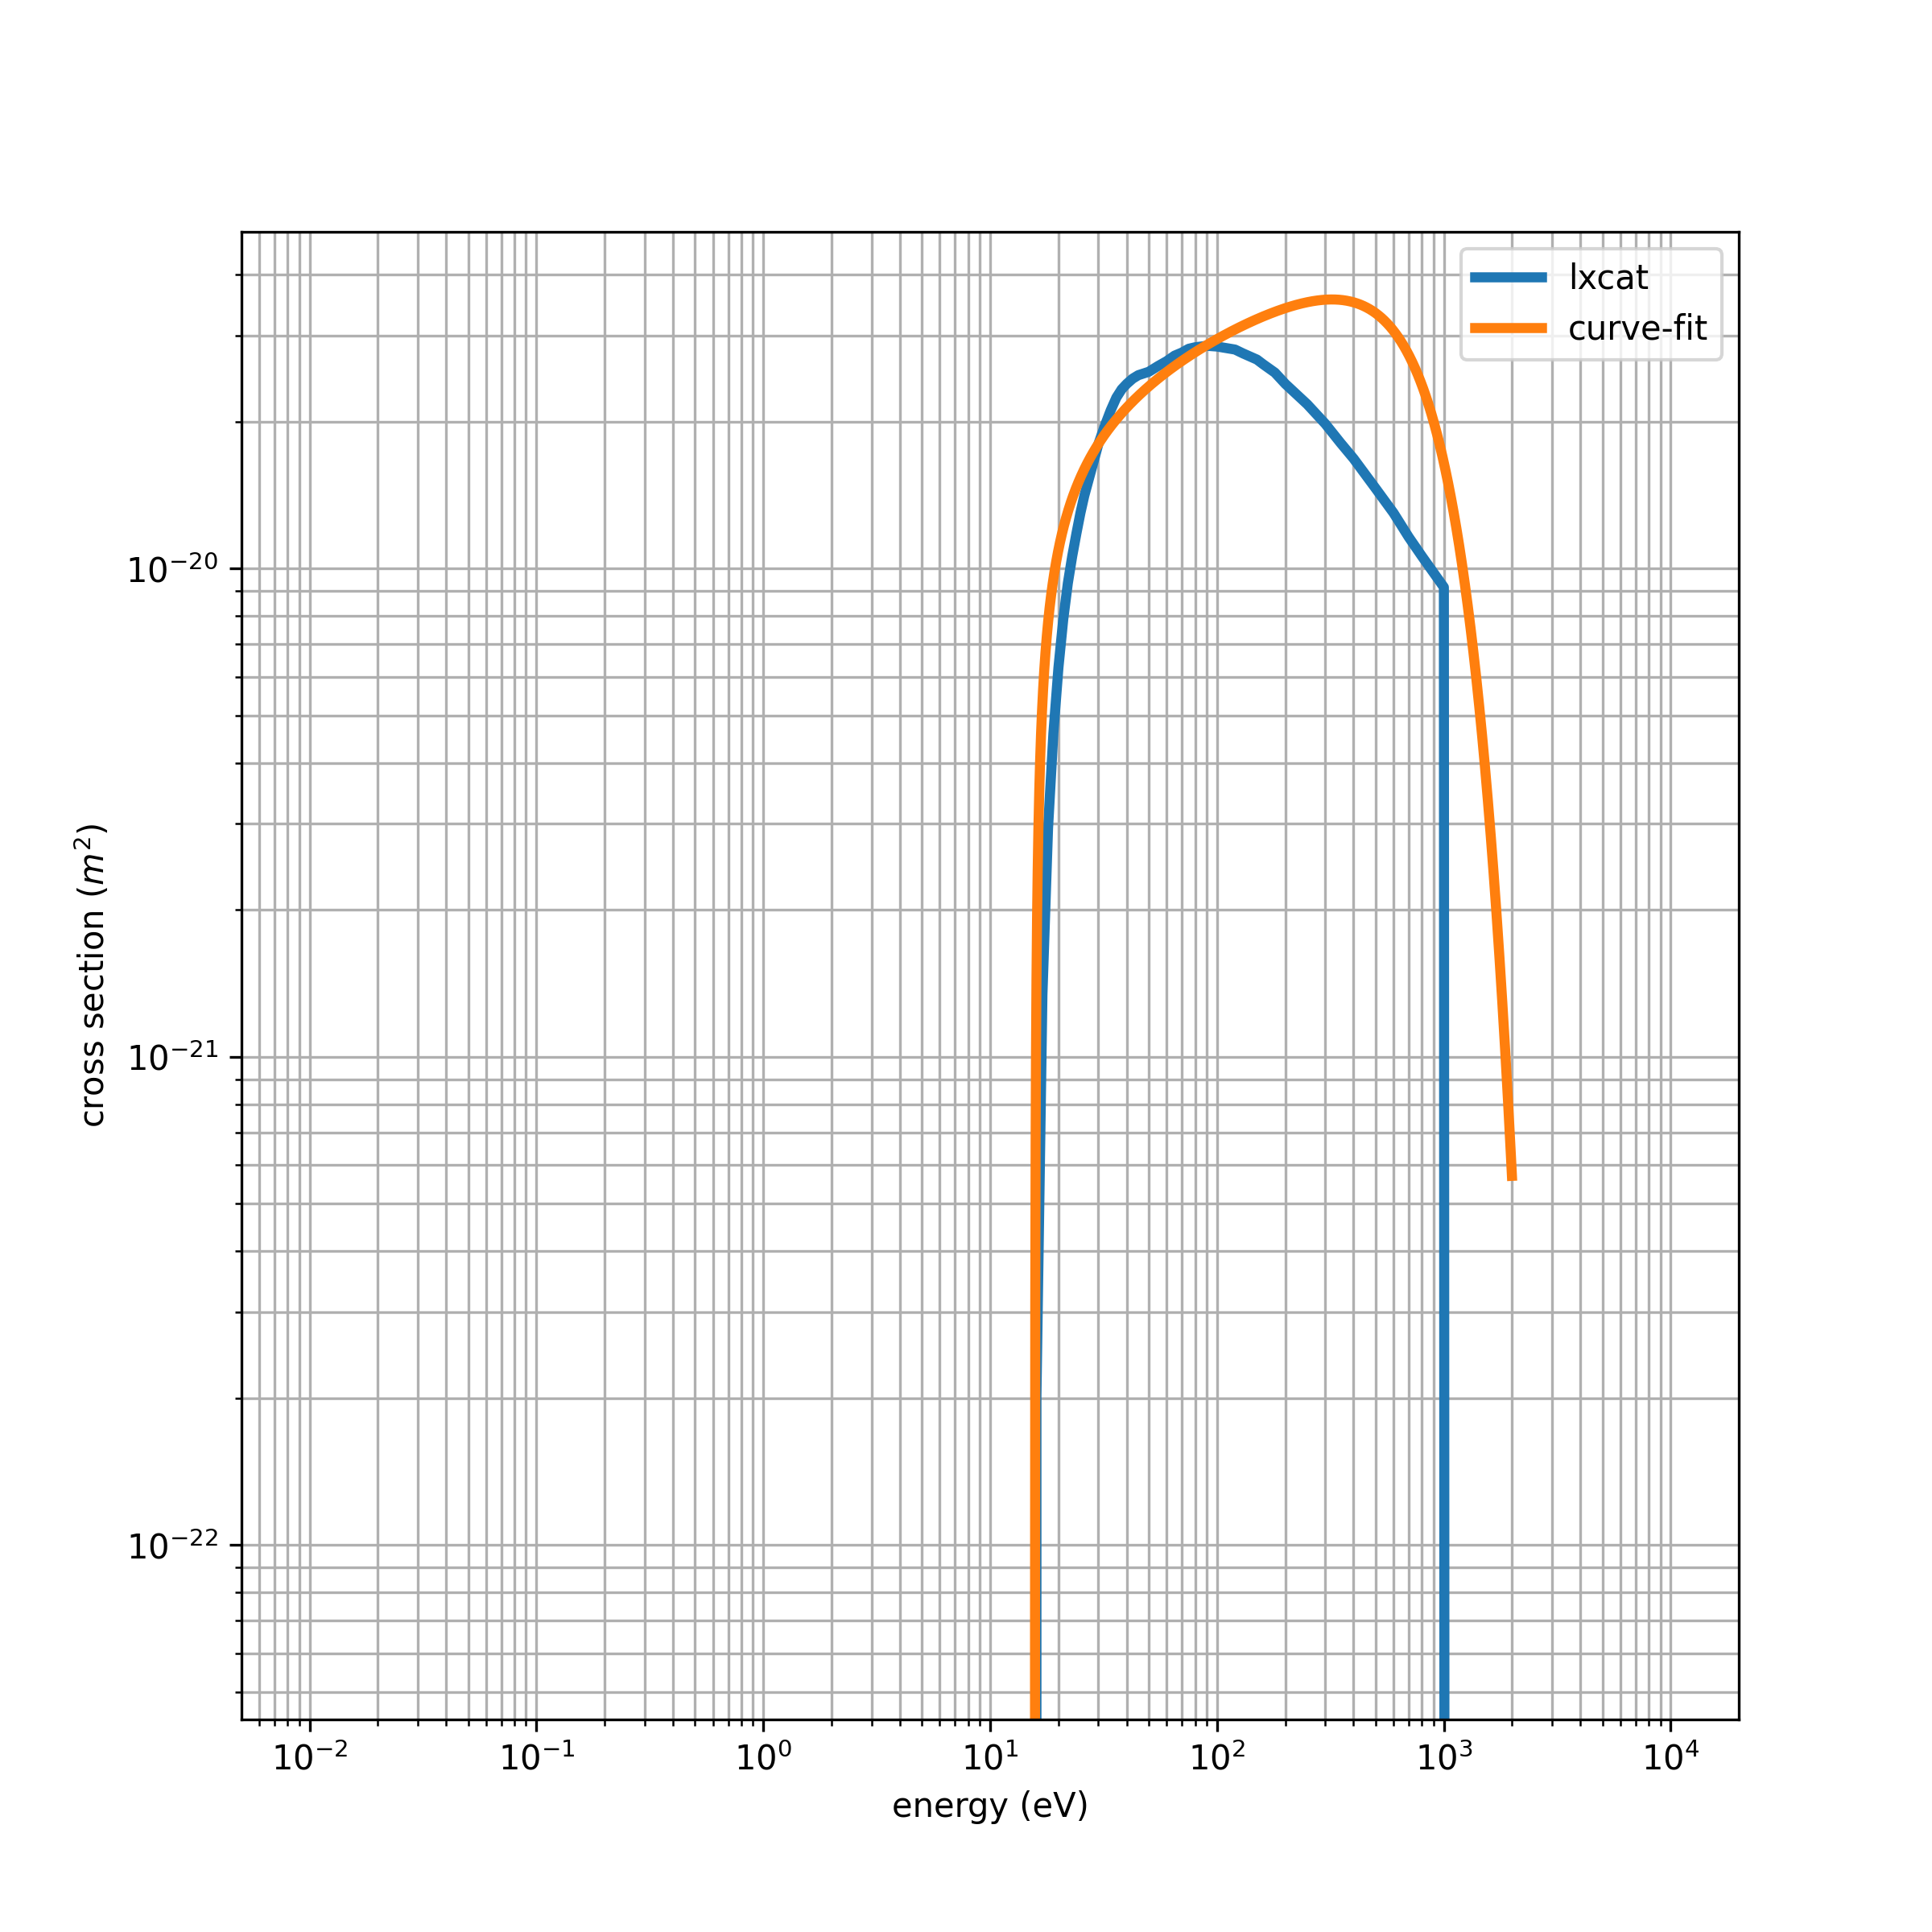
\includegraphics[width=0.36\textwidth]{fig/g2.png}
		\end{tabular}	
	\end{center}
\end{frame}


\begin{frame}
	\frametitle{Steady-state solution}
	\begin{itemize}
		\item With $\vect{E}\neq 0$, the normalized distribution function should reach a steady state. 
		$
		\displaystyle
		\quad
		\partial_t (\hat{f}) = -(u^T C \hat{f}) \hat{f} + (C-E)\hat{f} \text{ where } \hat{f}(\vect{v},t) = \frac{f(v,t)}{\myint_{R^3} f(\vect{v},t) \diff{\vect{v}}}
		$
		\item Numerical evolution of the normalized distribution result in a DAE with constraint $u^T \hat{f}-1=0 \forall t>0$
		\item Steady-state solution to the above can be achieved via solving below.  
		$
		\displaystyle
		\quad
		\partial_t (\hat{f}) = 0 \Rightarrow -(u^T C \hat{f}) \hat{f} + (C-E)\hat{f} =0
		$ with $u^T \hat{f}-1=0$
		\item For the work presented, we use steady-state solve, avoiding time integrator to reach the steady-state solution. 
	\end{itemize}
\end{frame}

\begin{frame}
	\frametitle{Bolsig+ code}
	\begin{itemize}
		\item Not an open-source code. 
		\item Solves the electron Boltzmann equation in uniform electric fields with two term approximation.
		$
		\displaystyle
		\quad
		f(\vect{v},t) = f_0(v, t) + f_1(v,t)\cos v_\theta
		$ 
		\item Use approximations to simplify the evaluation of the collision operator (i.e., less computational work for collision operator assembly)
		\item \textbf{Numerical method}: Use finite volume with, exponential scheme to construct solution at the cell boundaries.  
		\item The code is fast and stable for all the cases that we tried. 
	\end{itemize}
\end{frame}

\begin{frame}
	\frametitle{Comparison with Bolsig+}
	\begin{itemize}
		\item We use const E field aligned with z-axis. 
		\item Deploy (0,0) and (1,0) lm modes to match the expansion used in the Bolsig+ .
		\item Experiment with LXCAT data + other analytical cross-sections. 
		\item Steady-state solution is computed with steady-state equation without timestepping. 
		\item We used 4 quadrature points in all angular directions. 
		\begin{itemize}
			\item Global polynomials : used 200 quadrature points in the radial direction. 
			\item B-Splines : 2 quadrature points per knot interval, hence 2N quadrature points, where N is the number of splines used in the radial direction. 
		\end{itemize}
		\item Convergence is shown sweeping through the number of radial basis functions used. 
		\item Currently consider reactions, 
		\begin{itemize}
			\item G0 : $e + Ar \rightarrow e + Ar$
			\item G2 : $e + Ar \rightarrow 2e + Ar^+$
		\end{itemize}
	\end{itemize}
\end{frame}

\begin{frame}
	\frametitle{Maxwell polynomials}
	\only<+>{\textbullet~ E=1 V/m    \includegraphics[width=\textwidth]{fig/maxwell_vs_bolsig_g0_g2_E1.0_poly_maxwell_nr128_bscale1.0_sweeping_Nr.png}}
	\only<+>{\textbullet~ E=10 V/m   \includegraphics[width=\textwidth]{fig/maxwell_vs_bolsig_g0_g2_E10.0_poly_maxwell_nr128_bscale1.0_sweeping_Nr.png}}
	\only<+>{\textbullet~ E=100 V/m  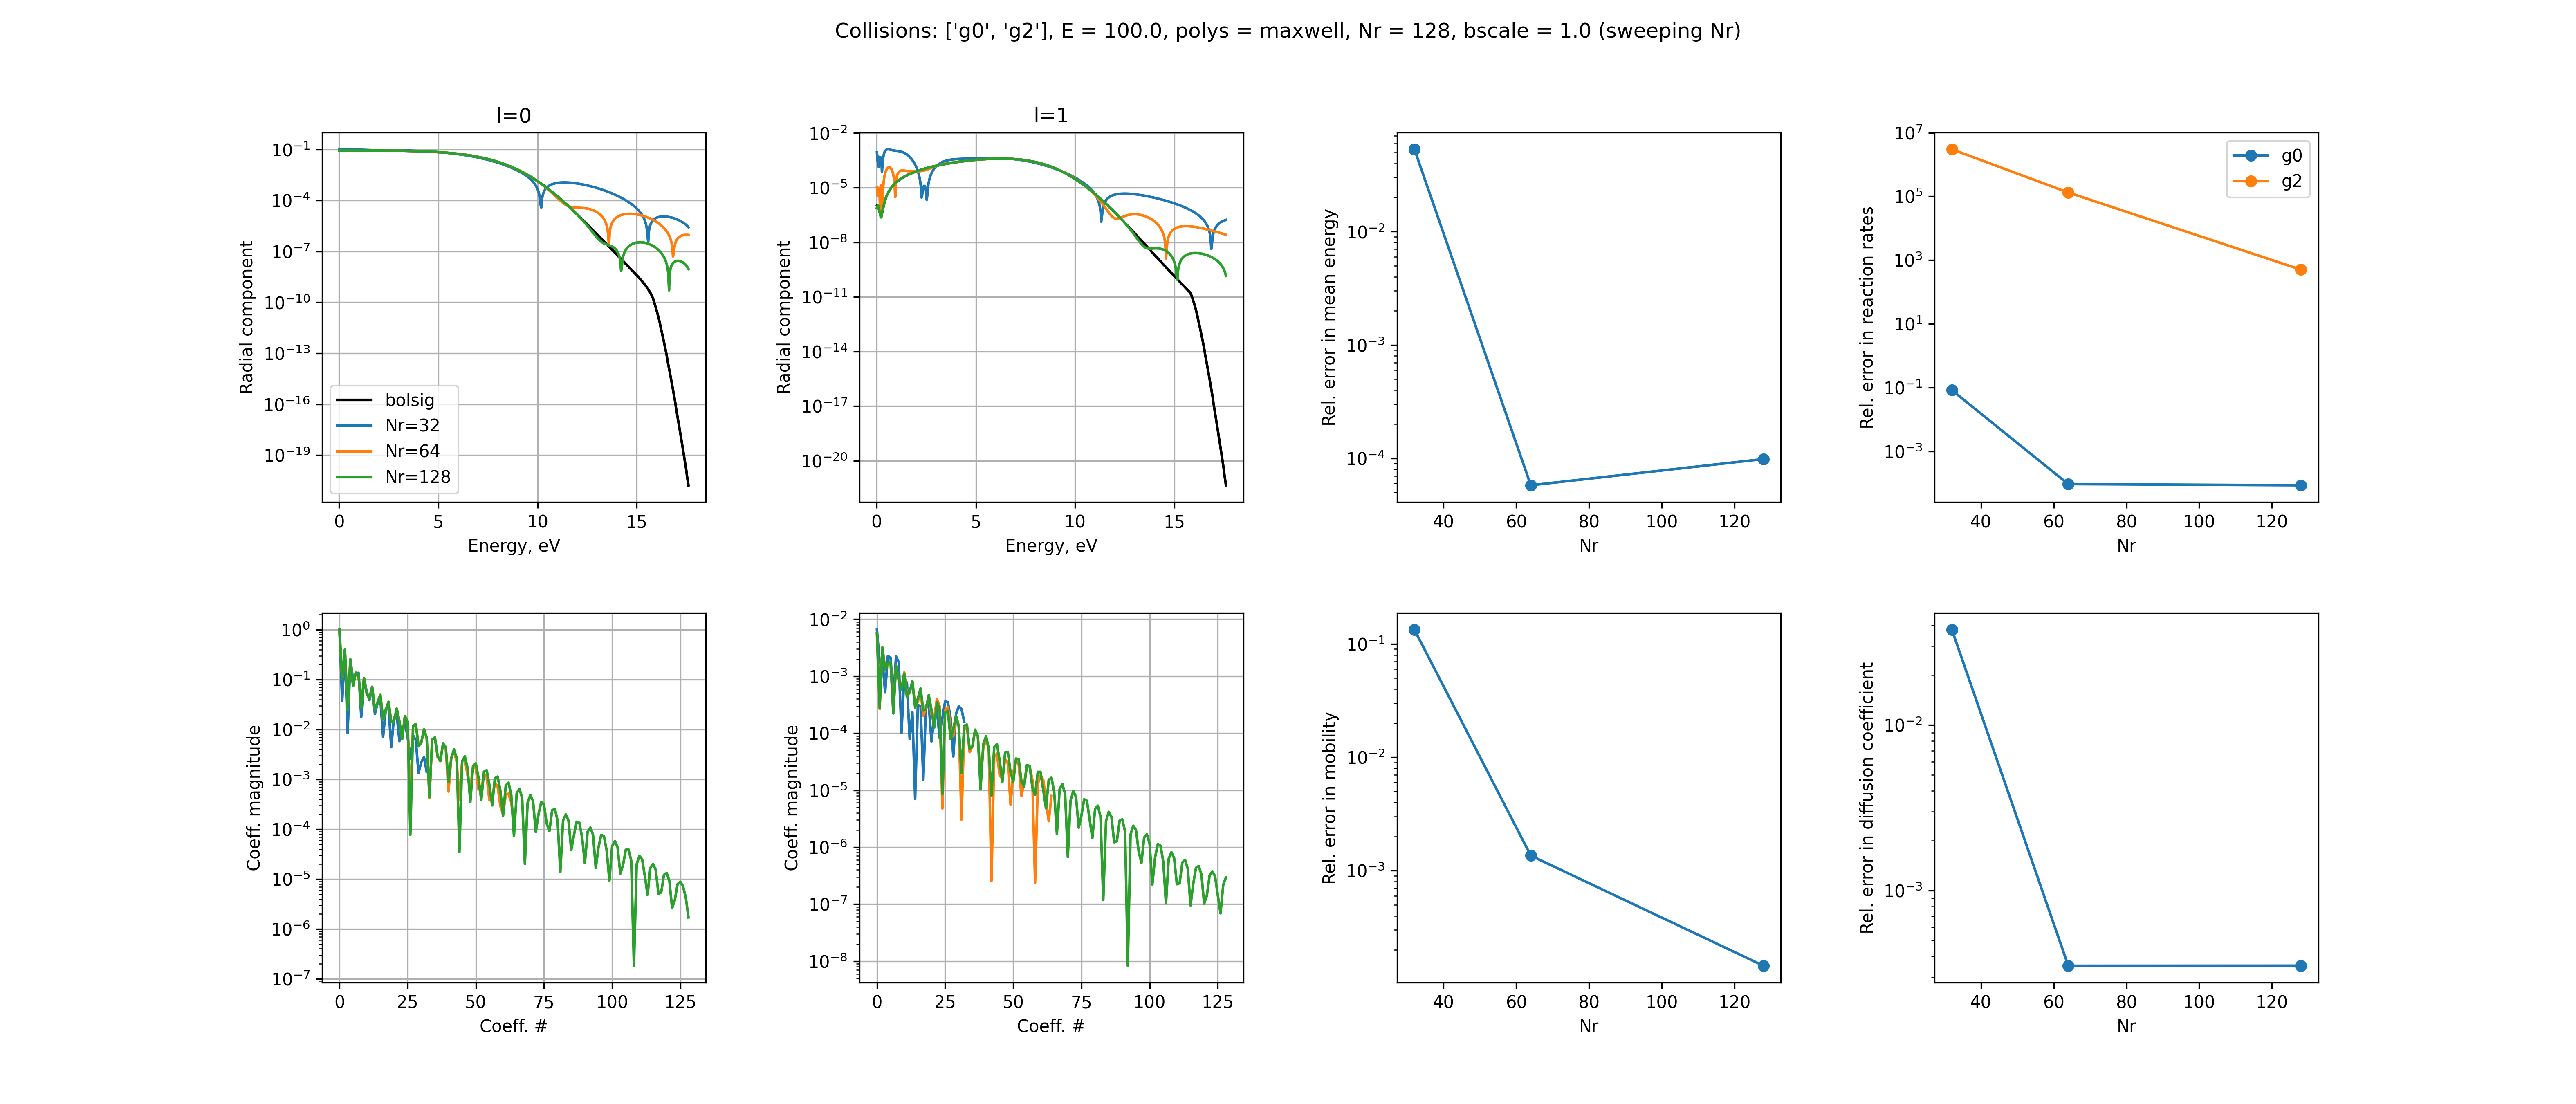
\includegraphics[width=\textwidth]{fig/maxwell_vs_bolsig_g0_g2_E100.0_poly_maxwell_nr128_bscale1.0_sweeping_Nr.png}}
	\only<+>{\textbullet~ E=500 V/m  \includegraphics[width=\textwidth]{fig/maxwell_vs_bolsig_g0_g2_E500.0_poly_maxwell_nr128_bscale1.0_sweeping_Nr.png}}
	\only<+>{\textbullet~ E=1000 V/m \includegraphics[width=\textwidth]{fig/maxwell_vs_bolsig_g0_g2_E1000.0_poly_maxwell_nr128_bscale1.0_sweeping_Nr.png}}
	\only<+>{\textbullet~ E=5000 V/m 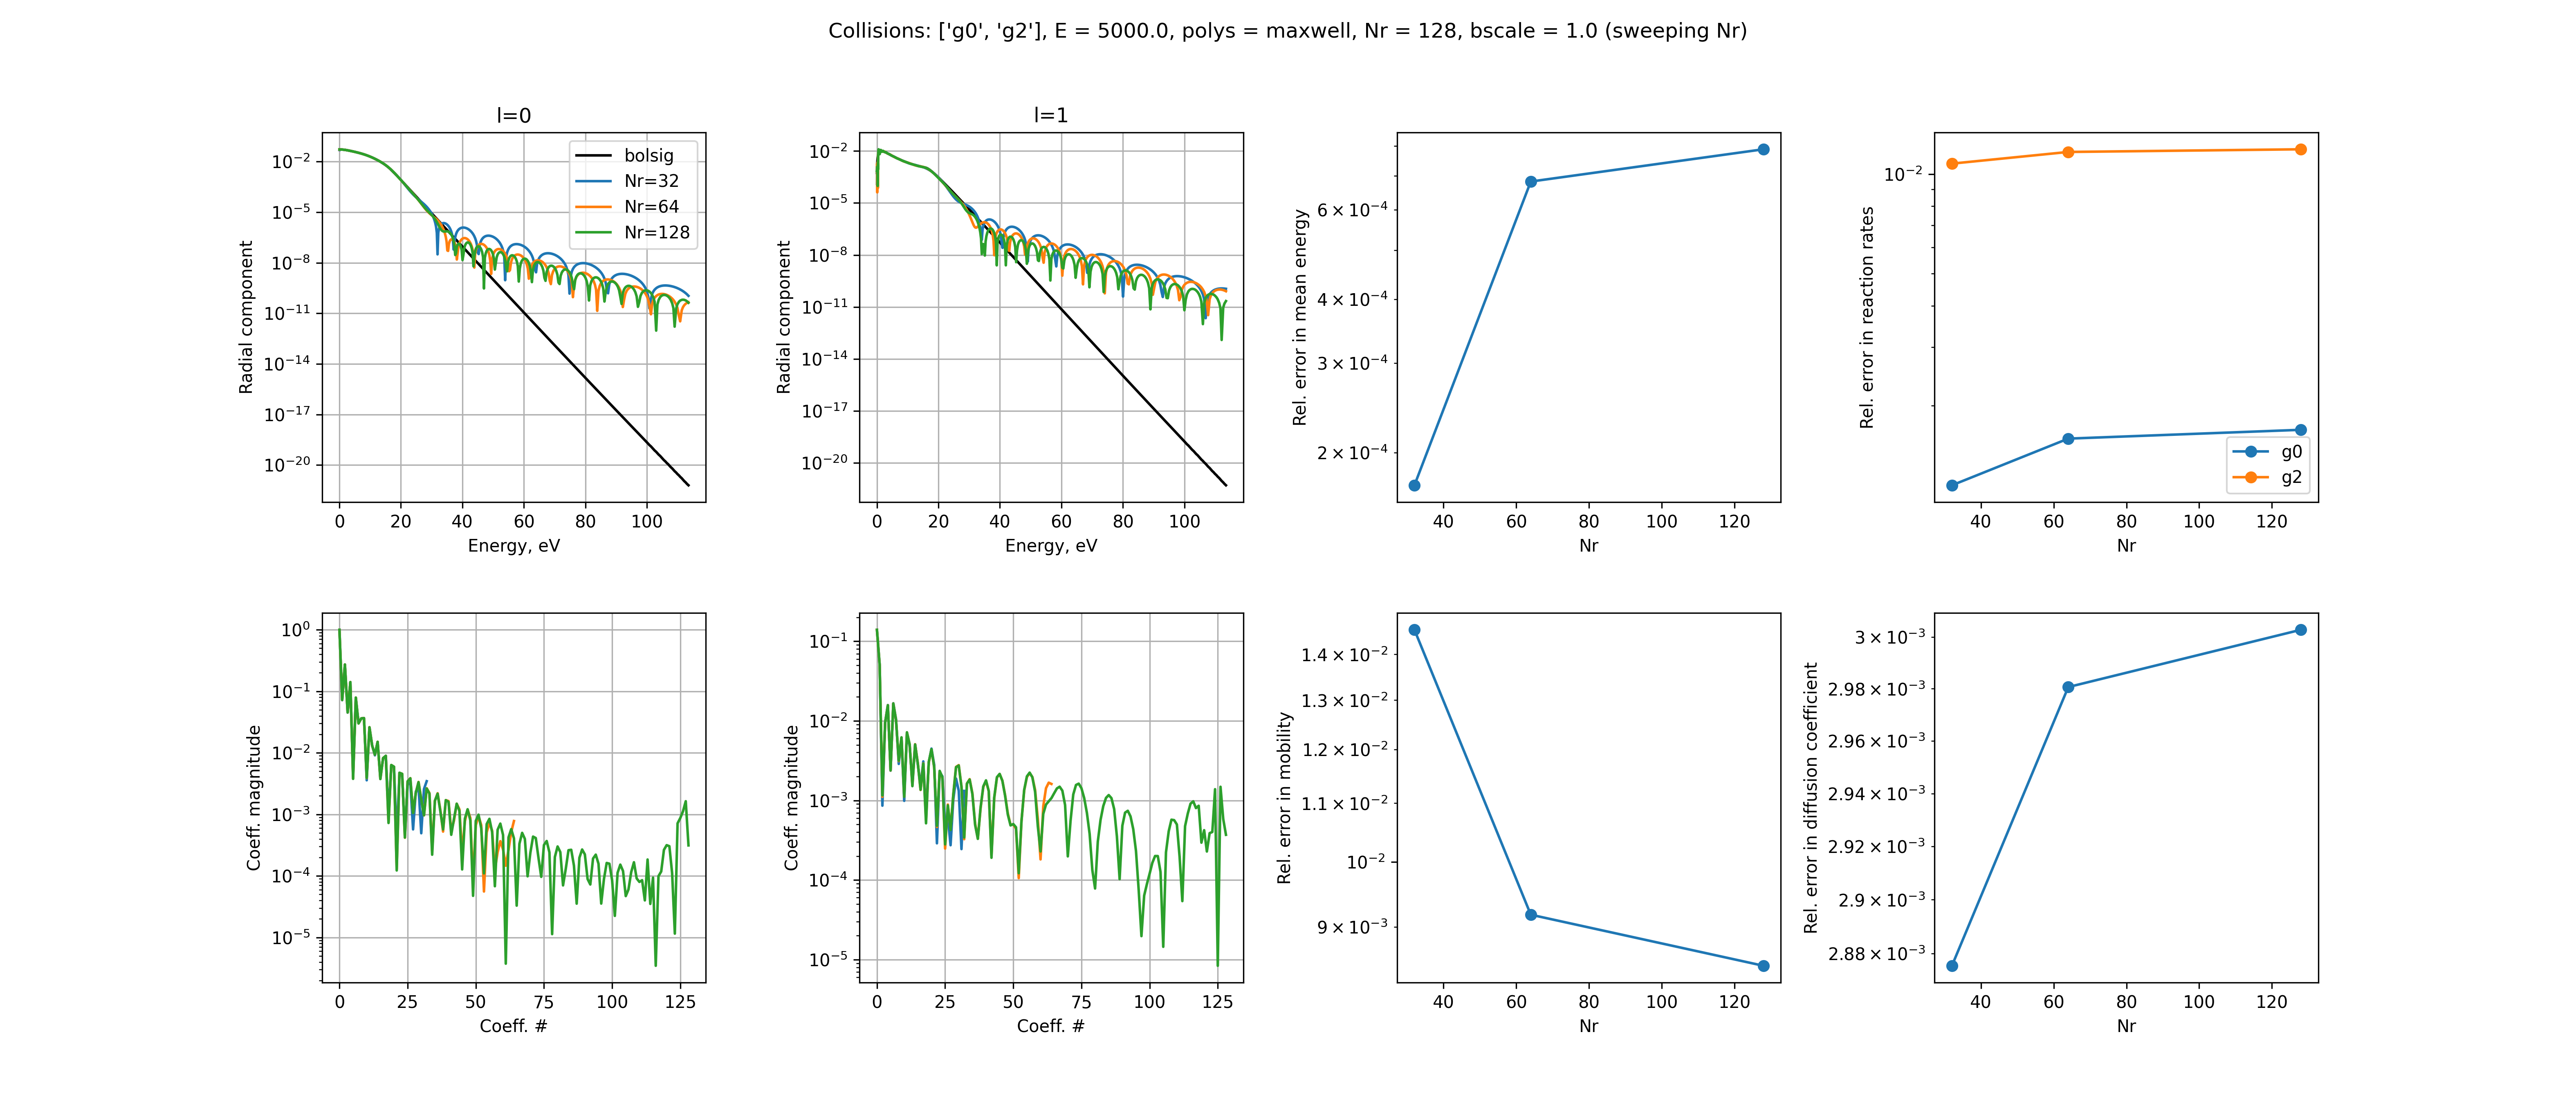
\includegraphics[width=\textwidth]{fig/maxwell_vs_bolsig_g0_g2_E5000.0_poly_maxwell_nr128_bscale1.0_sweeping_Nr.png}}
\end{frame}

% \begin{frame}
% 	\frametitle{Maxwell polynomials (in energy)}
% 	\begin{center}
% 		\only<+>{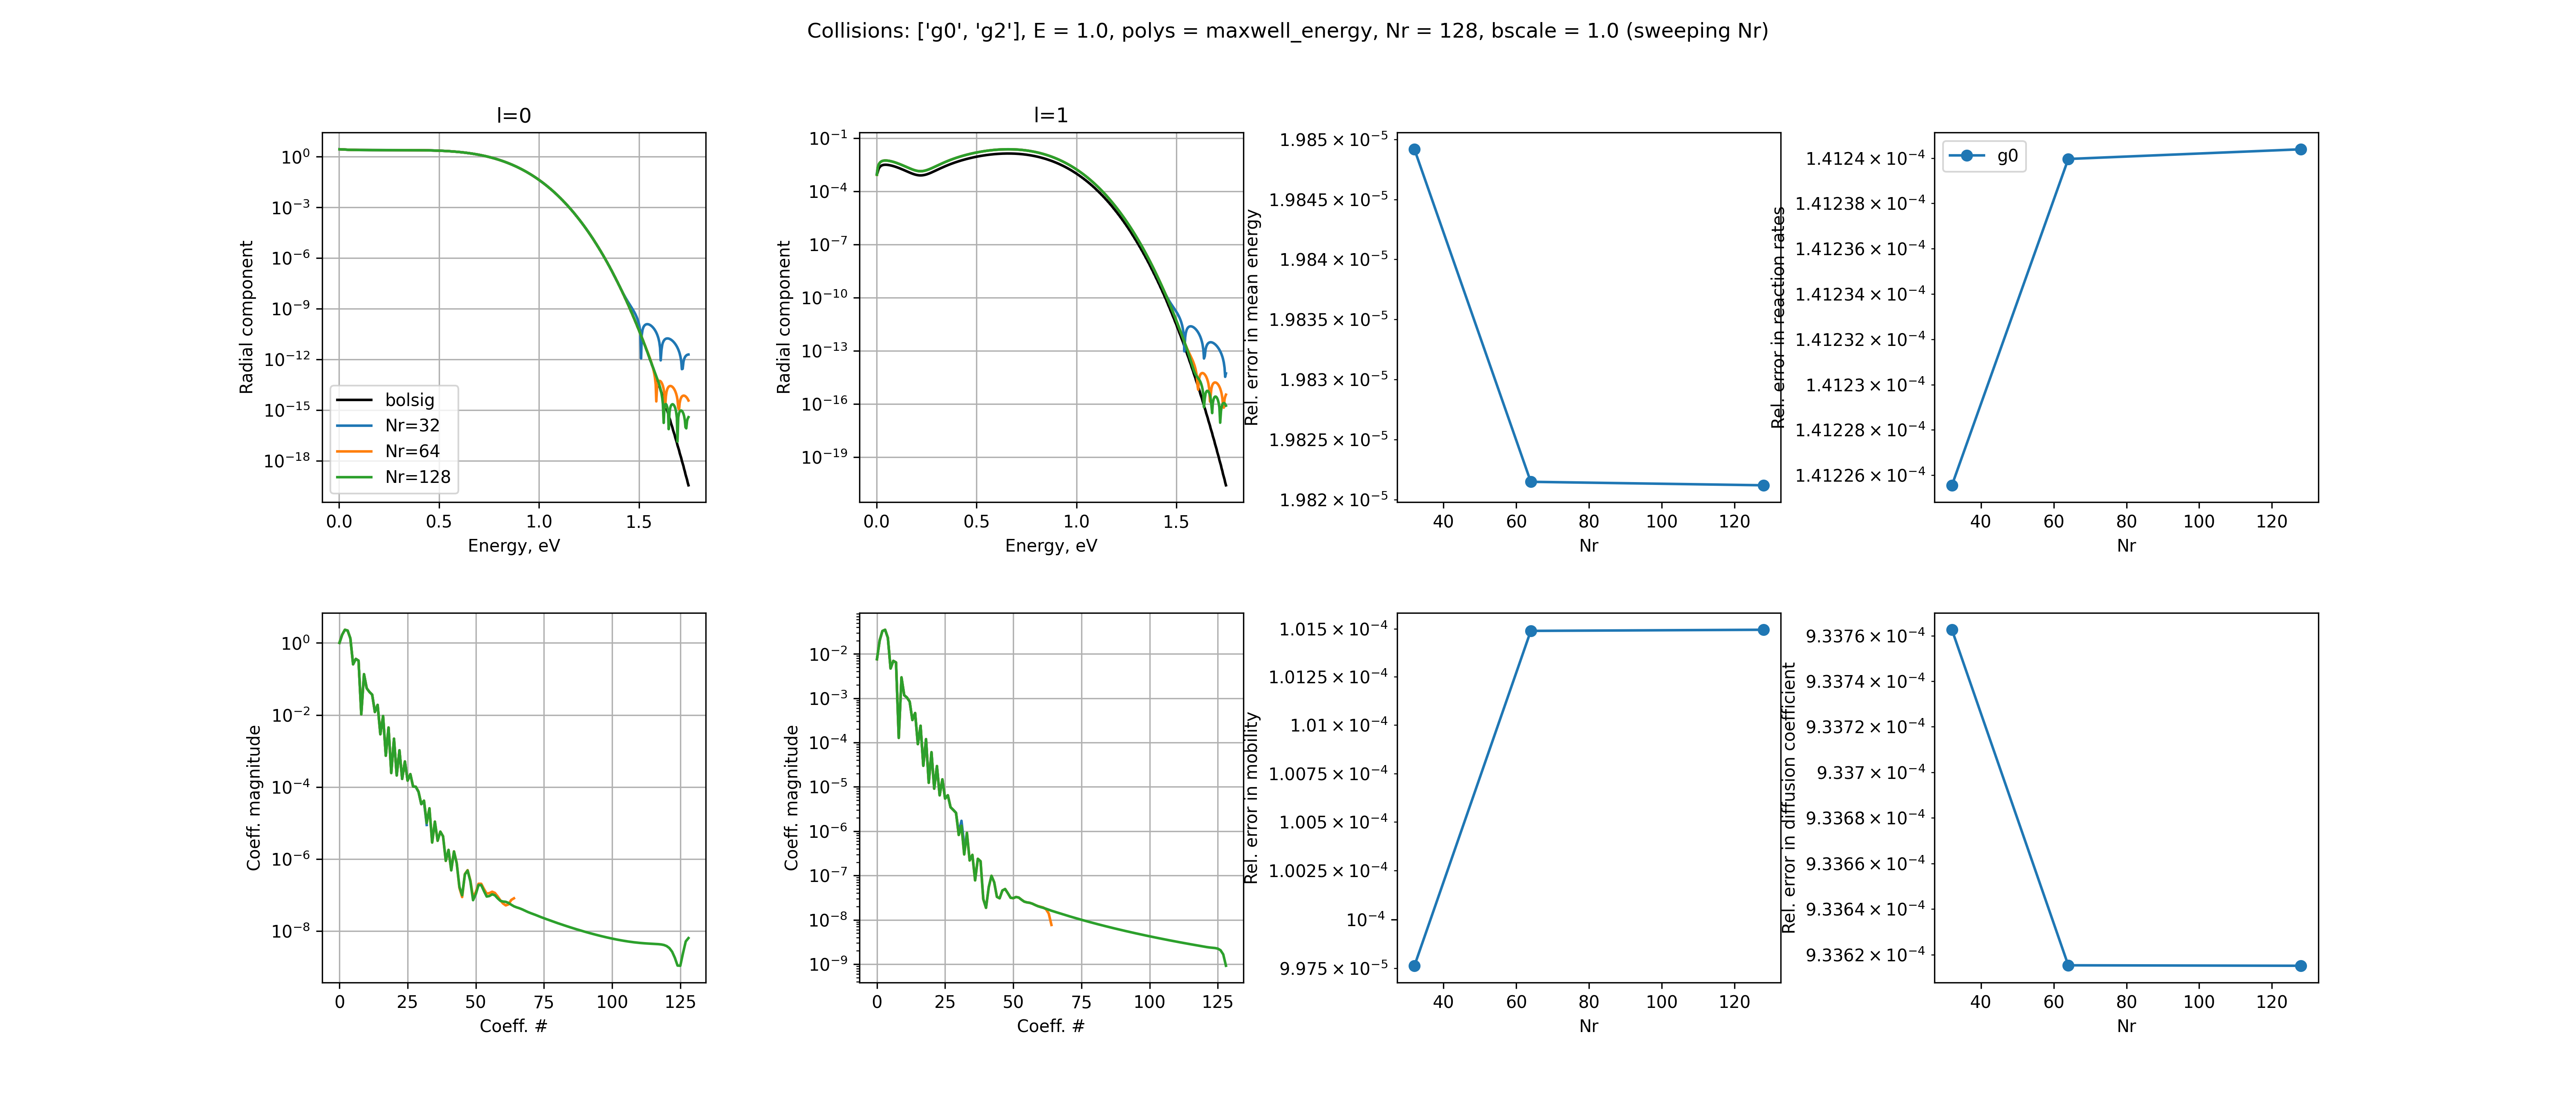
\includegraphics[width=\textwidth]{fig/maxwell_vs_bolsig_g0_g2_E1.0_poly_maxwell_energy_nr128_bscale1.0_sweeping_Nr.png}}
% 		\only<+>{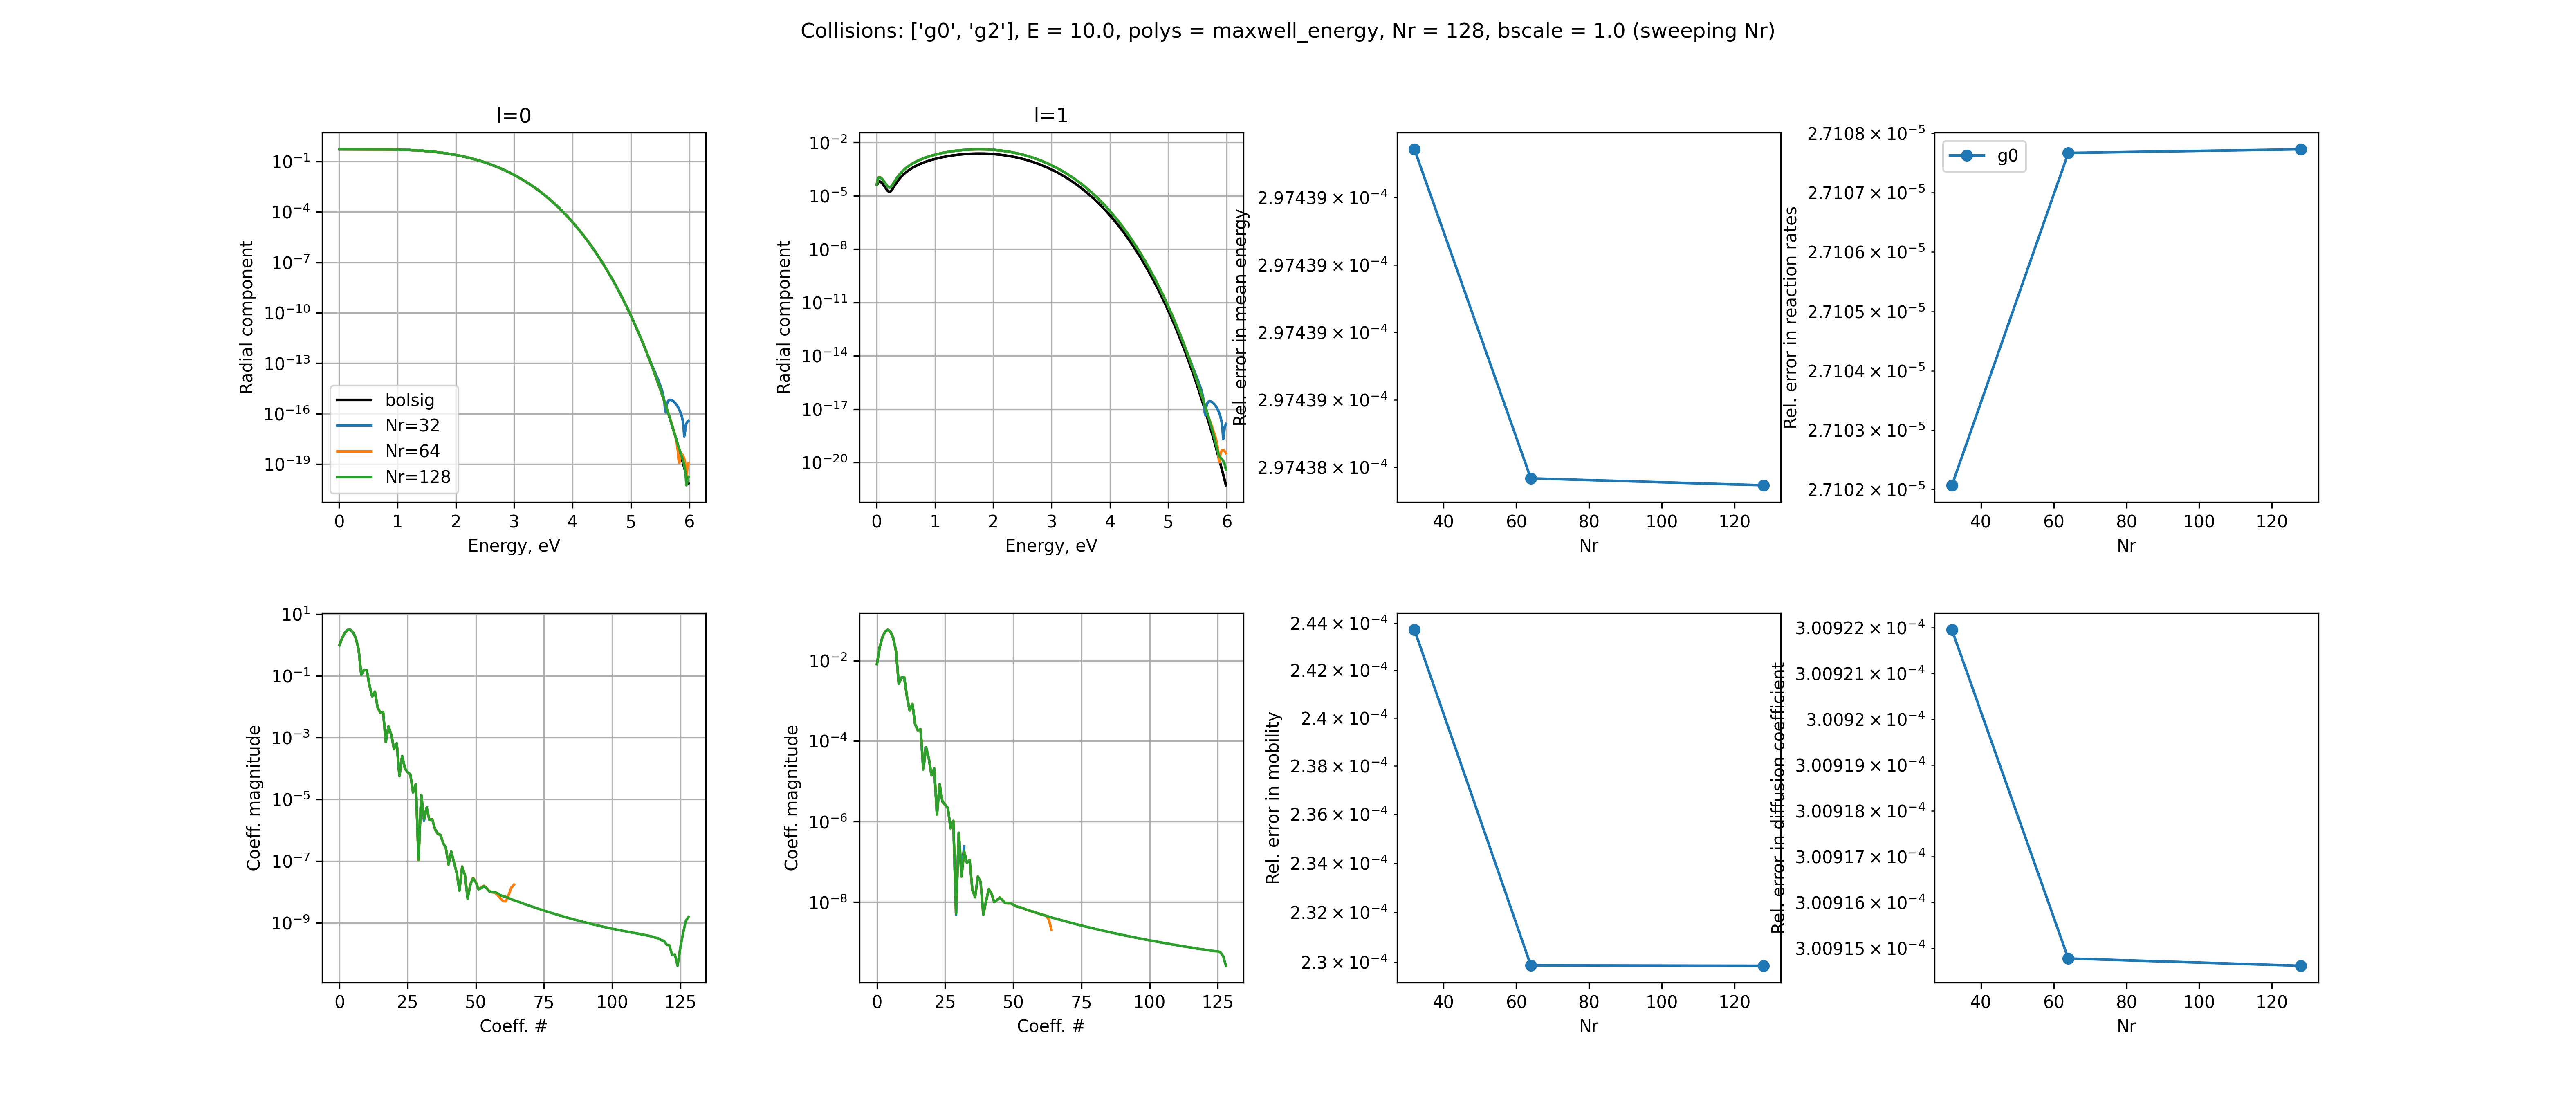
\includegraphics[width=\textwidth]{fig/maxwell_vs_bolsig_g0_g2_E10.0_poly_maxwell_energy_nr128_bscale1.0_sweeping_Nr.png}}
% 		\only<+>{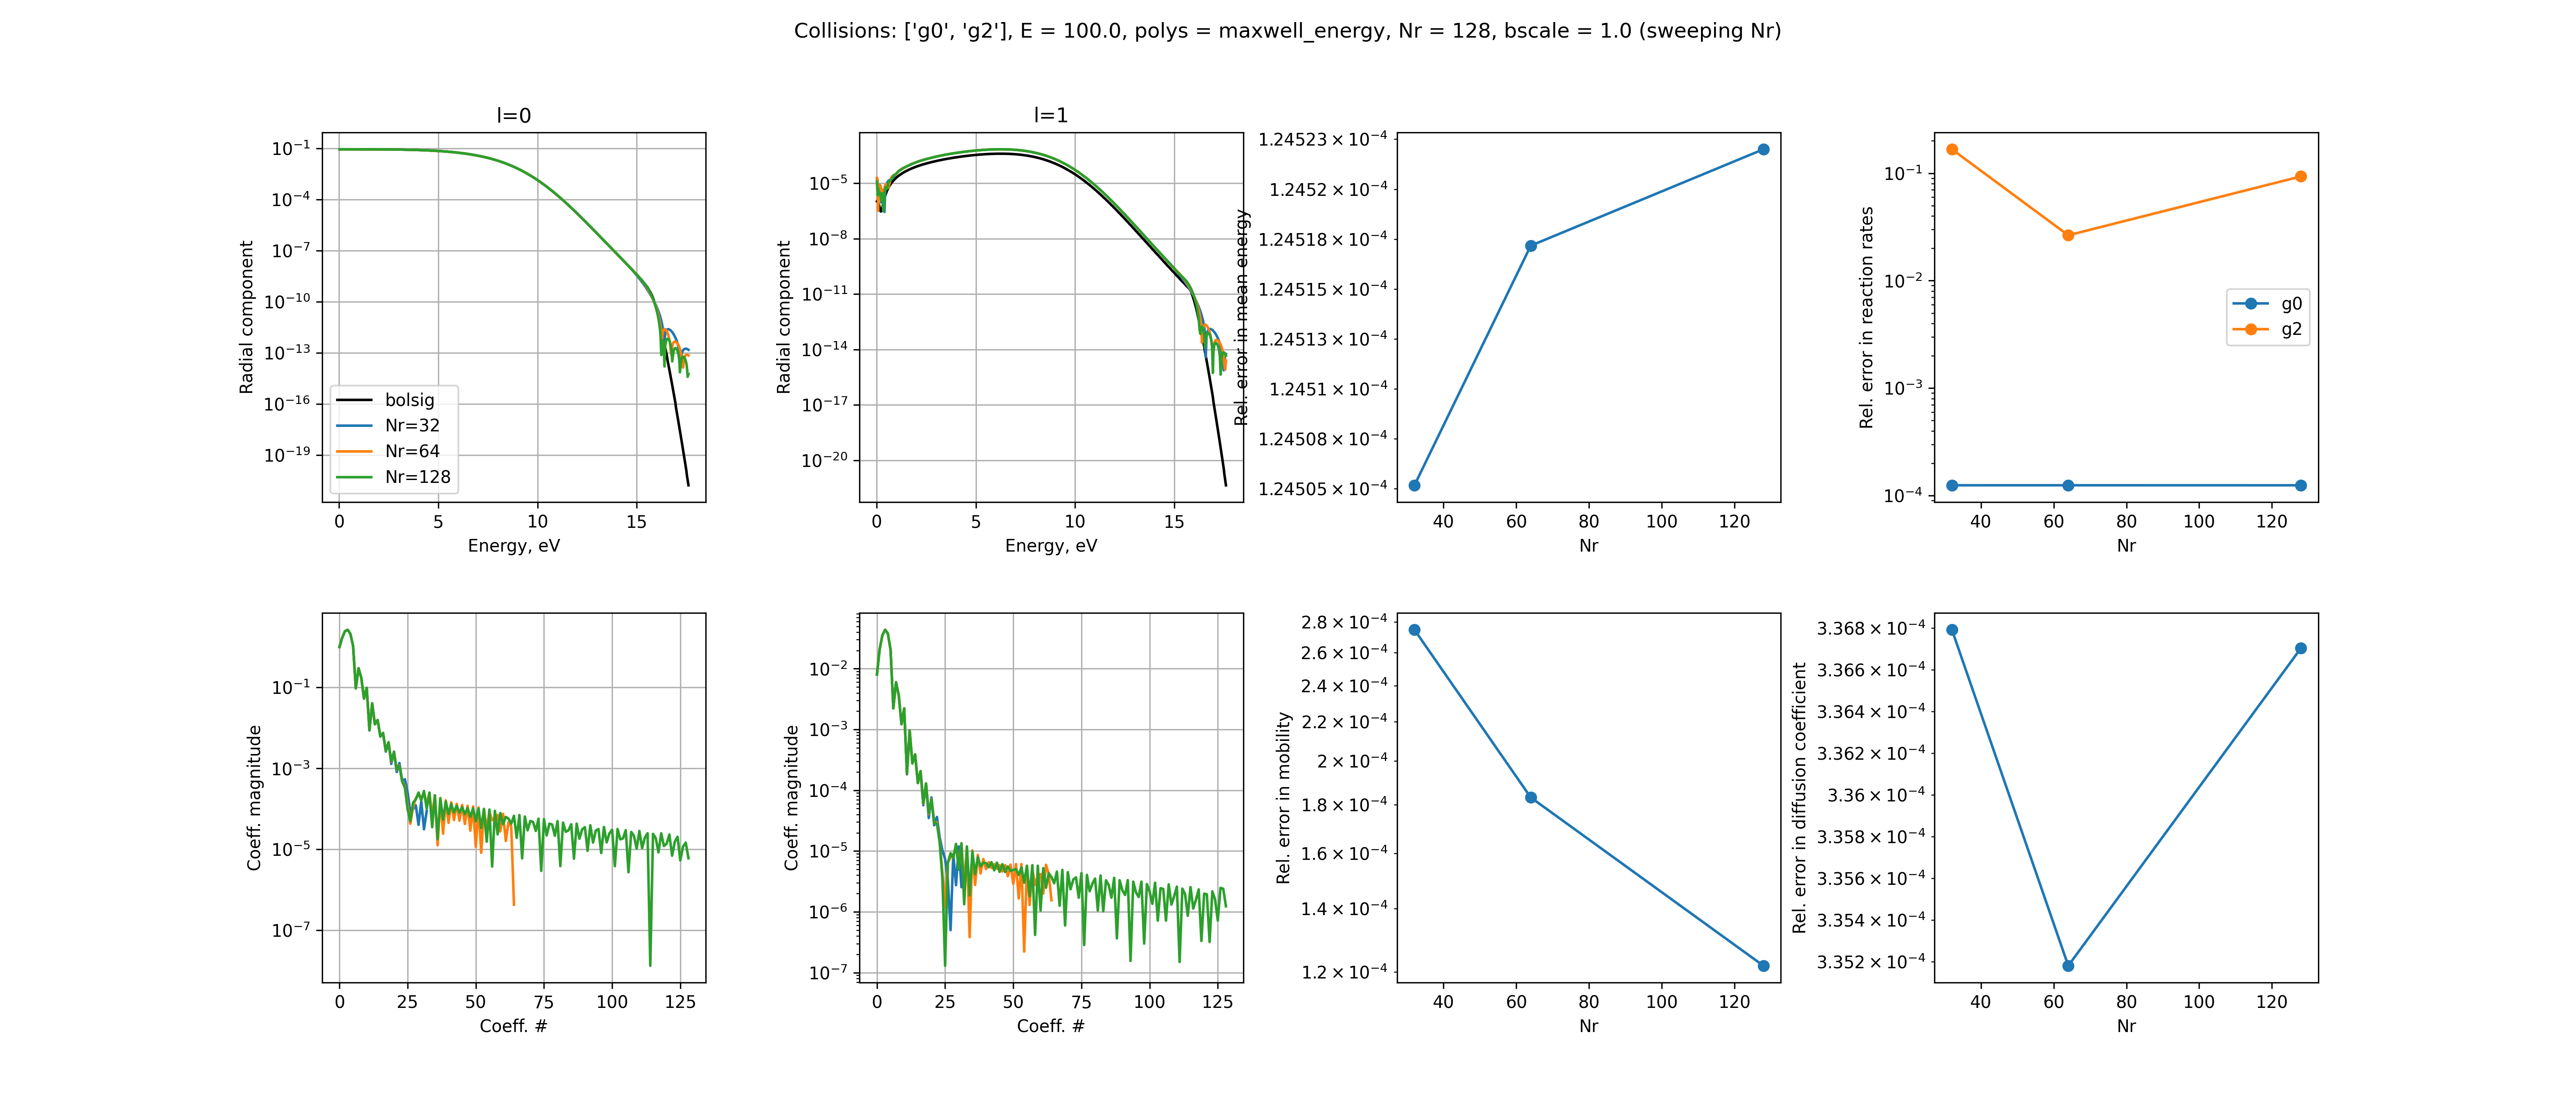
\includegraphics[width=\textwidth]{fig/maxwell_vs_bolsig_g0_g2_E100.0_poly_maxwell_energy_nr128_bscale1.0_sweeping_Nr.png}}
% 		% \only<+>{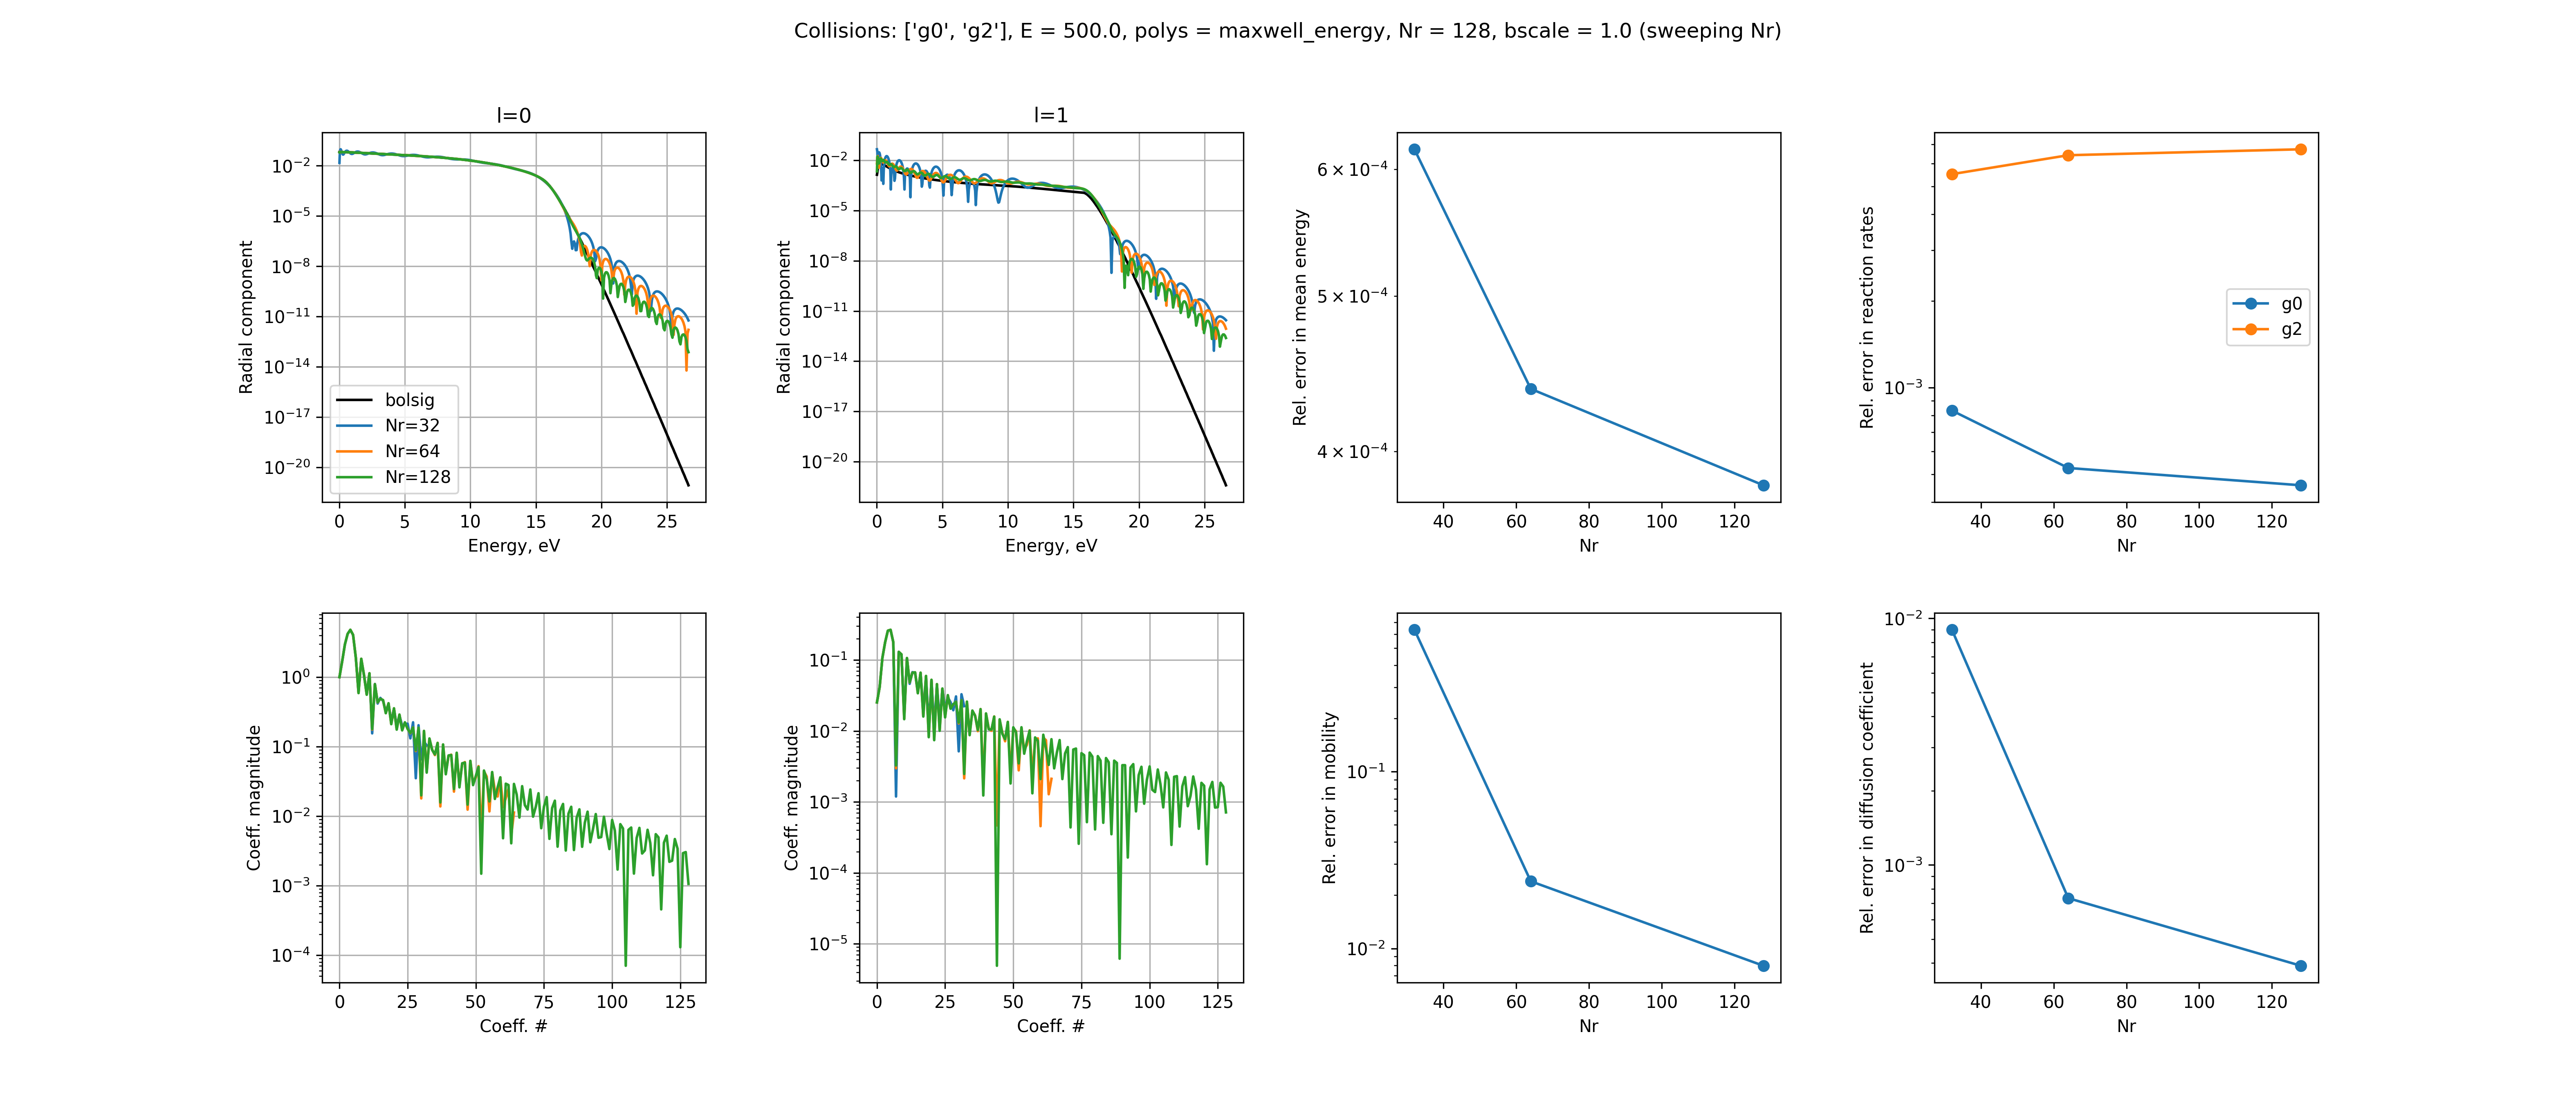
\includegraphics[width=\textwidth]{fig/maxwell_vs_bolsig_g0_g2_E500.0_poly_maxwell_energy_nr128_bscale1.0_sweeping_Nr.png}}
% 		% \only<+>{\includegraphics[width=\textwidth]{fig/maxwell_vs_bolsig_g0_g2_E1000.0_poly_maxwell_energy_nr128_bscale1.0_sweeping_Nr.png}}
% 	\end{center}
% \end{frame}

\begin{frame}
	\frametitle{Linear B-splines}
	\only<+>{\textbullet~ E=1 V/m    \includegraphics[width=\textwidth]{fig/bspline_cg_vs_bolsig_g0_g2_E1.0_poly_bspline_sp_1_nr256_bscale1.0_sweeping_Nr.png}}
	\only<+>{\textbullet~ E=10 V/m   \includegraphics[width=\textwidth]{fig/bspline_cg_vs_bolsig_g0_g2_E10.0_poly_bspline_sp_1_nr256_bscale1.0_sweeping_Nr.png}}
	\only<+>{\textbullet~ E=100 V/m  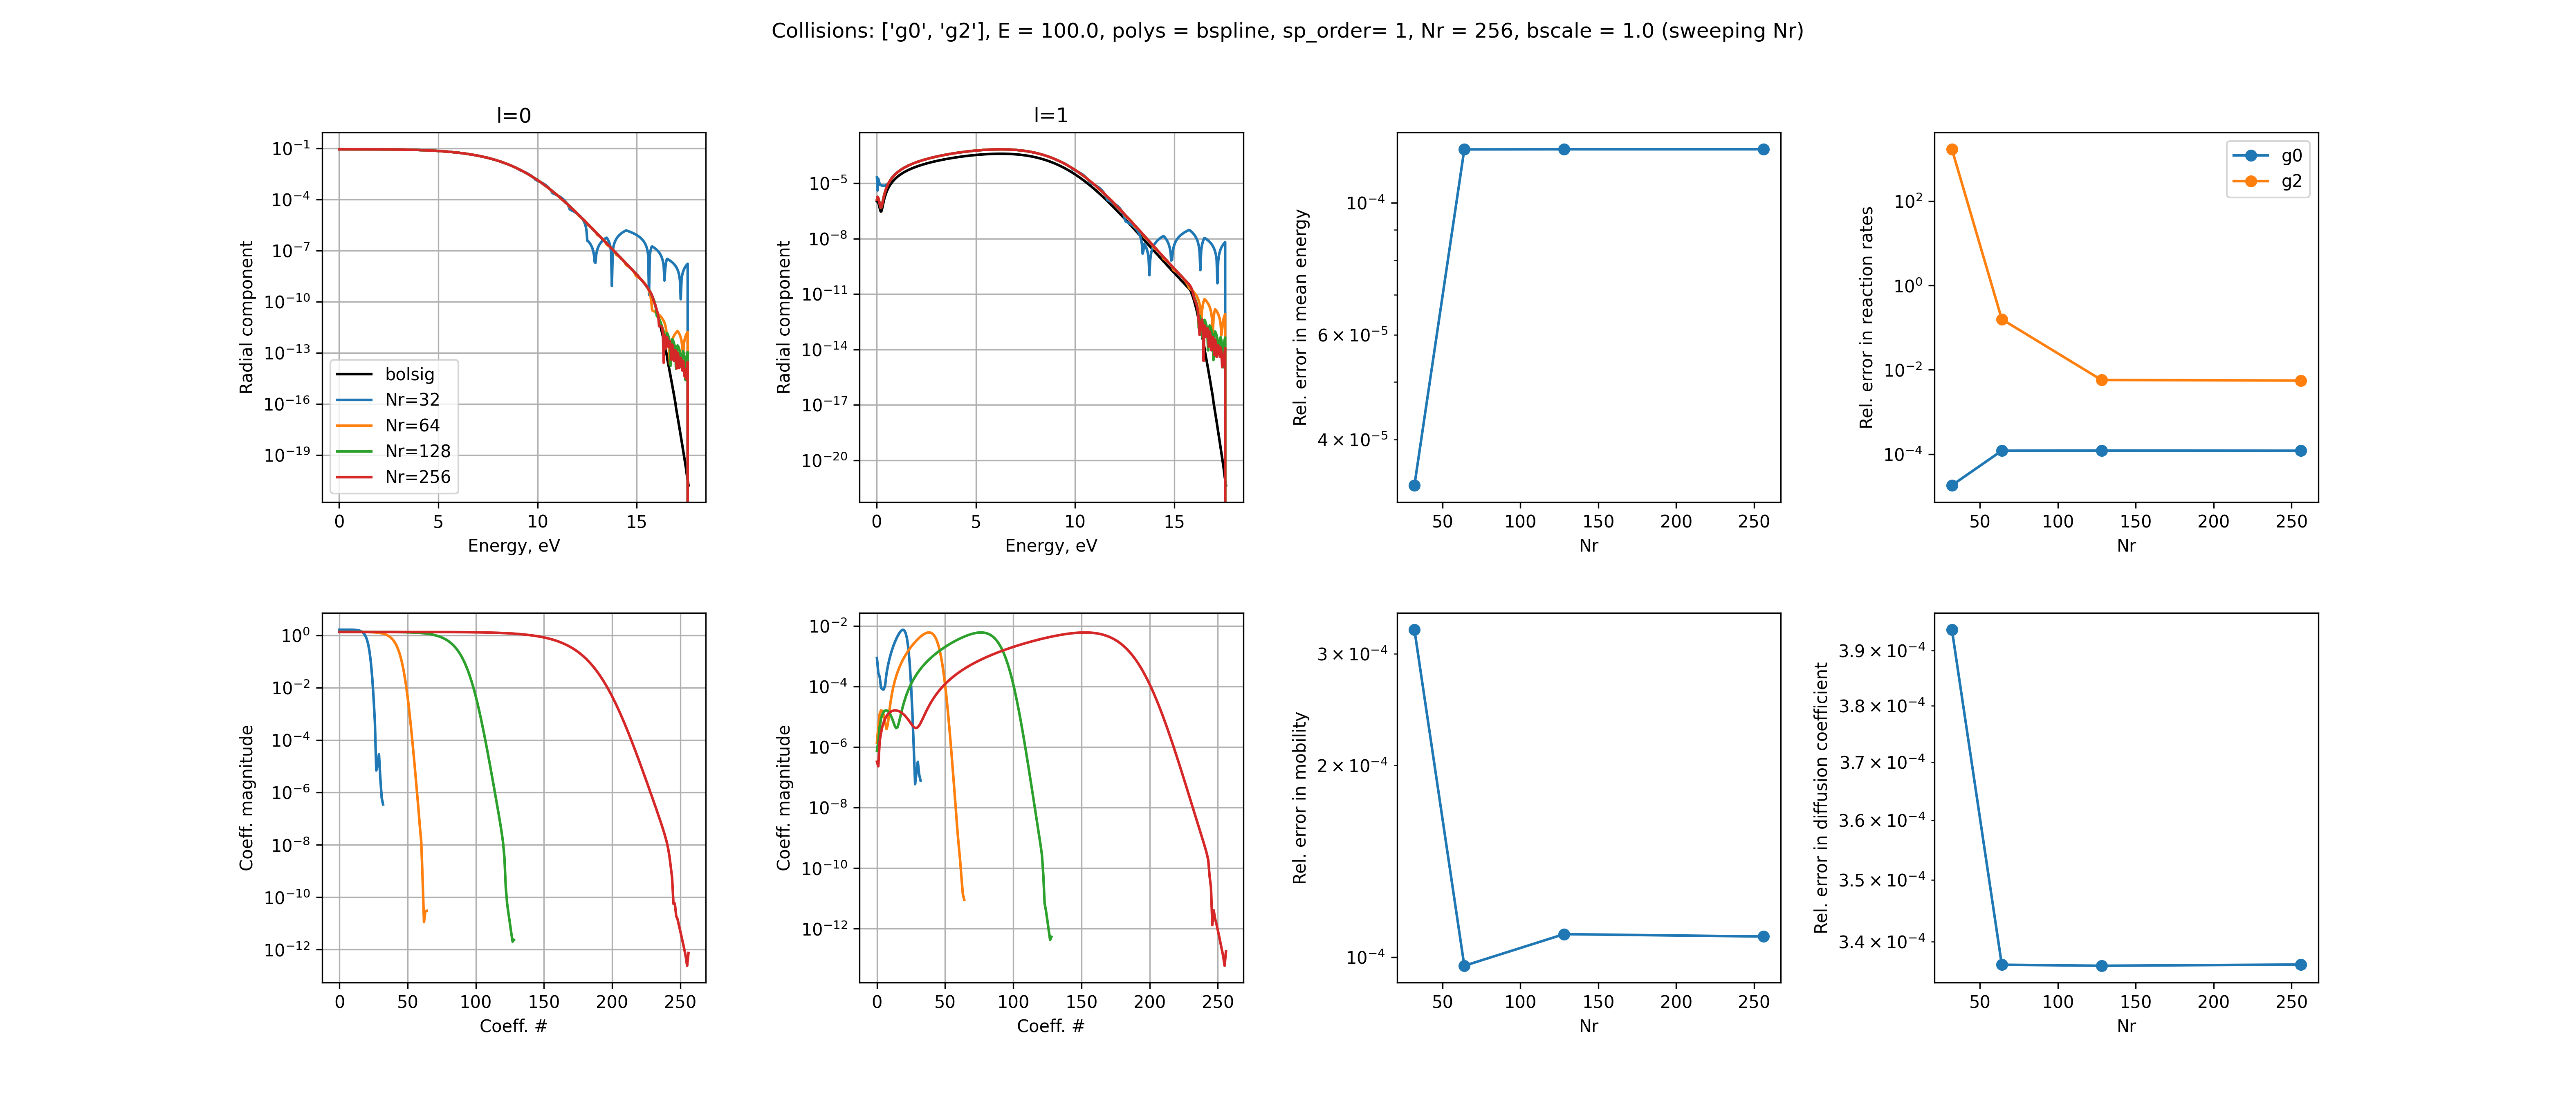
\includegraphics[width=\textwidth]{fig/bspline_cg_vs_bolsig_g0_g2_E100.0_poly_bspline_sp_1_nr256_bscale1.0_sweeping_Nr.png}}
	\only<+>{\textbullet~ E=500 V/m  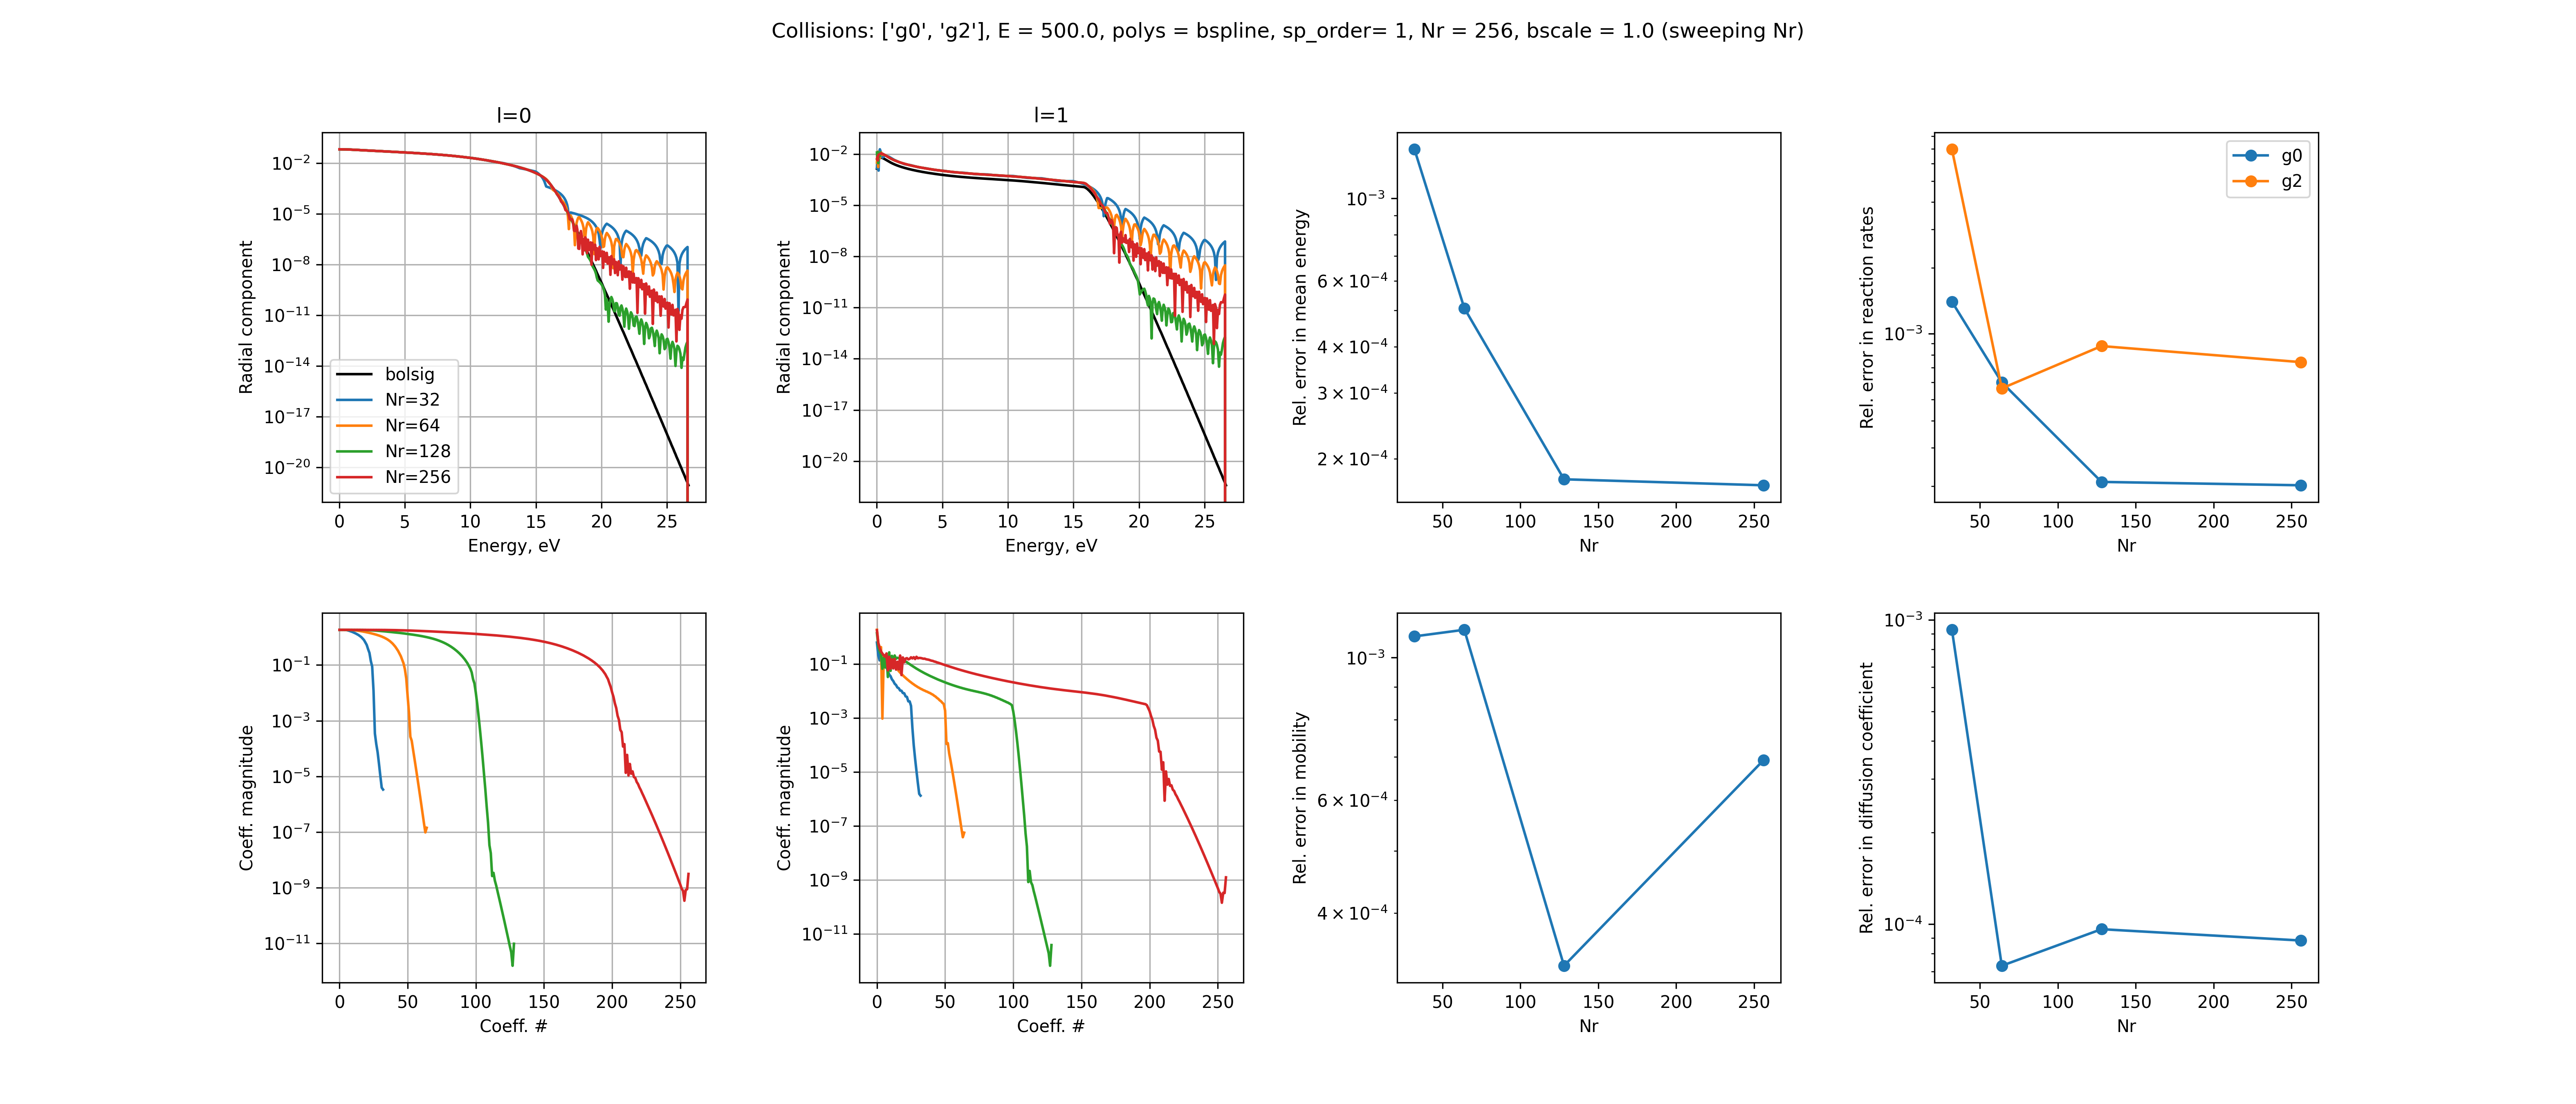
\includegraphics[width=\textwidth]{fig/bspline_cg_vs_bolsig_g0_g2_E500.0_poly_bspline_sp_1_nr256_bscale1.0_sweeping_Nr.png}}
	\only<+>{\textbullet~ E=1000 V/m 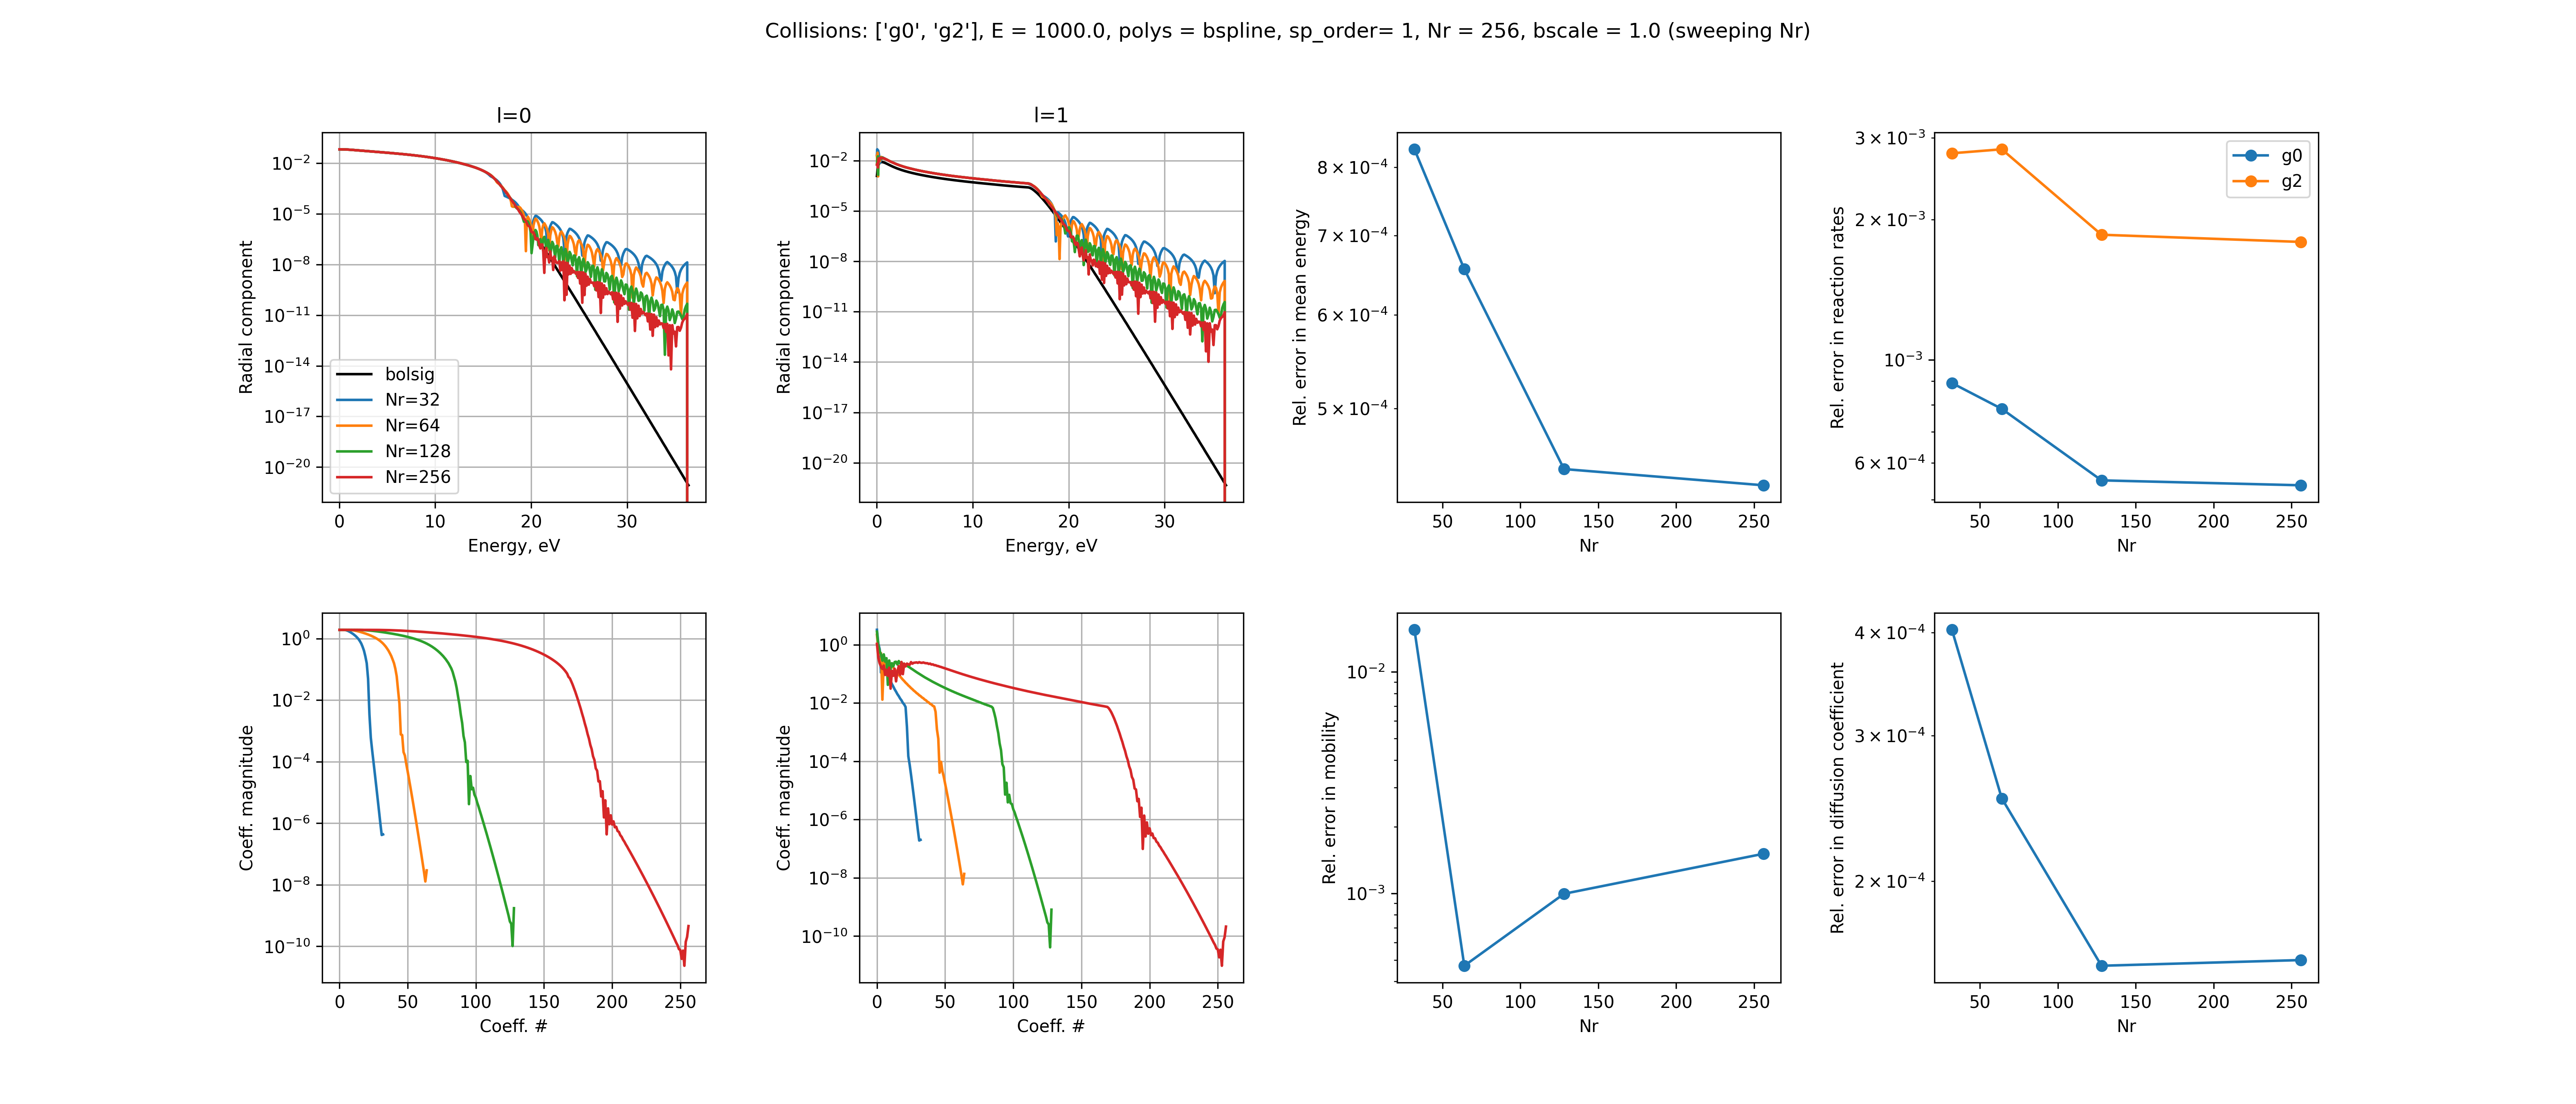
\includegraphics[width=\textwidth]{fig/bspline_cg_vs_bolsig_g0_g2_E1000.0_poly_bspline_sp_1_nr256_bscale1.0_sweeping_Nr.png}}
	\only<+>{\textbullet~ E=5000 V/m 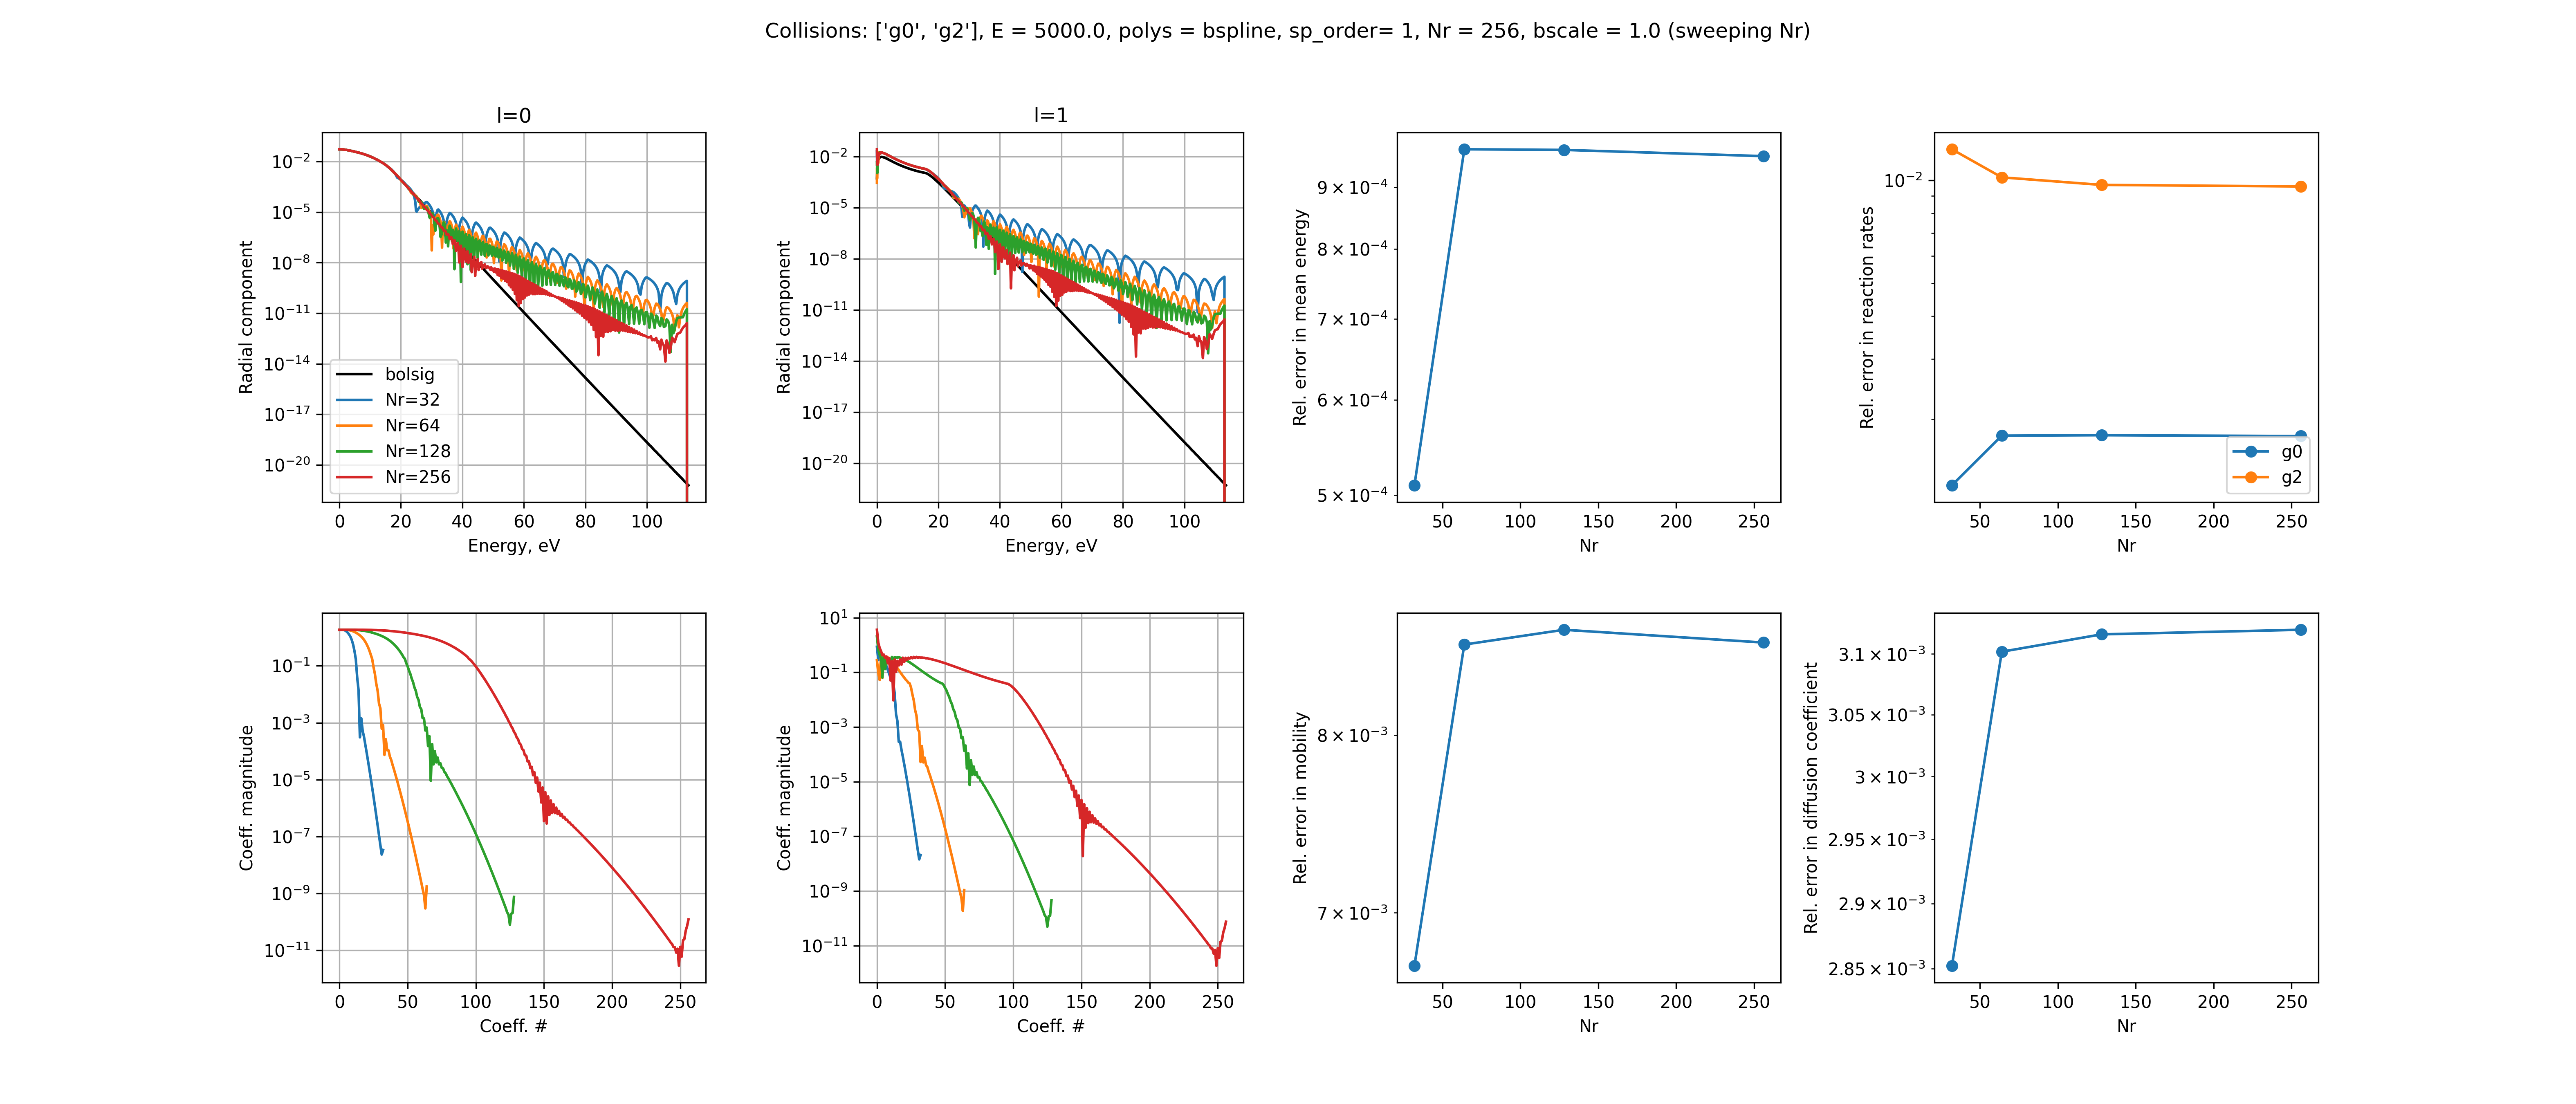
\includegraphics[width=\textwidth]{fig/bspline_cg_vs_bolsig_g0_g2_E5000.0_poly_bspline_sp_1_nr256_bscale1.0_sweeping_Nr.png}}
\end{frame}

\begin{frame}
	\frametitle{Maxwell with smooth cross-sections}
	\only<+>
	{
		\begin{itemize}
			\item Maxwell with constant G0 cross-section data
		\end{itemize}
		\includegraphics[width=\textwidth]{fig/maxwell_vs_bolsig_g0Const_E100.0_poly_maxwell_nr128_bscale1.0_sweeping_Nr.png}
	}
	\only<+>
	{
		\begin{itemize}
			\item Maxwell with constant G0 cross-section with smooth G2 cross-section. 
		\end{itemize}
		\includegraphics[width=\textwidth]{fig/maxwell_vs_bolsig_g0Const_g2Regul_E100.0_poly_maxwell_nr128_bscale1.0_sweeping_Nr.png}
	}

\end{frame}

\begin{frame}
	\frametitle{Observations}
	\begin{itemize}
		\item All cases have tail oscillations, with LXCAT cross-section data. 
		\begin{itemize}
			\item Discontinuities in ionization cross-section data
			\item Linear B-Splines advection is equivalent to central finite differencing. Therefore, upwinding issues ?
		\end{itemize}
		\item Global polynomials (Maxwell, Laguerre)
		\begin{itemize}
			\item Pros
			\begin{itemize}
				\item Spectral convergence
				\item Work well with highly smoothed cross-sections
			\end{itemize}
			\item Cons
			\begin{itemize}
				\item With LXCAT data tails are not well resolved. 
				\item Struggle to capture sharp variations in $f$.
			\end{itemize}
		\end{itemize}
		\item Local approximations with B-Splines
		\begin{itemize}
			\item Pros
			\begin{itemize}
				\item Flexibility
				\item With LXCAT data tails are comparatively better than global polynomials. 
			\end{itemize}
			\item Cons
			\begin{itemize}
				\item Linear convergence
				\item Require higher number of polynomials.
			\end{itemize}
		\end{itemize}
	\end{itemize}
\end{frame}

\begin{frame}[fragile]
	\frametitle{Discontinuties in cross-section data}
	\begin{itemize}
		\item Cross-sections can have discontinuities at threshold energy ($\epsilon_{0}$) for reactions.   $\Rightarrow$ makes $f$ non-smooth at $\epsilon_{0}$.
		\item Deploy discontinuous Galerkin method to handle discontinuity at $\epsilon_{0}$.
	\end{itemize}
	\begin{figure}
		\centering
		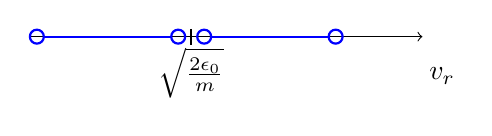
\begin{tikzpicture}
			\draw[black, ->](0,-0.0) -- (5,-0.0) node at (5.25, -0.5) {$v_r$};
			\draw[thick, blue, o-o] (0,0)--(2,0);
			\draw[thick, blue, o-o] (2.125,0)--(4.0,0);
			\draw[thick, black,-] (2.06,0.1)--(2.06,-0.1);
			\node at(2.06,-0.46) {$\sqrt{\frac{2\epsilon_0}{m}}$};
		\end{tikzpicture}
	\end{figure}
	\begin{itemize}
		\item In spherical coordinates, advection direction is non-trivial, $lm$ modes are coupled together. 
		$\displaystyle
		\quad
		\partial_tf_{qs} + E A^{qs}_{lm} \partial_v f_{lm} +E B^{qs}_{lm} \frac{1}{v}f_{lm}  = C^{qs}_{lm}f_{lm}
		$
		\item Evolve the diagonalized system with, $A^{qs}_{lm} = Q \Lambda^{qs}_{lm} Q^T$.
		$\displaystyle
		\quad
		\partial_t y_{qs} +E\Lambda^{qs}_{lm} \partial_v y_{lm} +E Q^T B^{qs}_{lm} \frac{1}{v} Q y_{lm} = Q^T C^{qs}_{lm} Q y_{lm}
		$
		\item Upwinding at $\sqrt{\frac{2\epsilon_0}{m}}$ is performed according to the  sign of $(\Lambda^{qs}_{lm})$ diagonal entries. For example l=0,1 m=0 case,  
		\begin{itemize}
			\item $y_{0,0}= \frac{1}{\sqrt{2}}\of{f_{0,0} + f_{1,0}}$ advection from left to right in radial direction
			\item $y_{1,0}= \frac{1}{\sqrt{2}}\of{f_{0,0} - f_{1,0}}$ advection from right to left in radial direction
		\end{itemize}
	\end{itemize}
	
\end{frame}

\begin{frame}
	\frametitle{DG with linear B-Splines}
	\begin{center}
		\includegraphics[width=0.85\textwidth]{fig/bspline_dg_vs_bolsig_g0_g2_E100.0_poly_bspline_sp_1_nr256_bscale1.0_sweeping_Nr.png}
	\end{center}
	\pause
	\begin{itemize}
		\item \textbf{Path forward}: Try Chebyshev with DG can help with the tail oscillations ??
	\end{itemize}
\end{frame}

\begin{frame}
	\begin{center}
		\onslide<+->\Large Questions ? \\
		\onslide<+>\Large Thank You. 
	\end{center}
\end{frame}

\end{document}

